%%%%%%%%%%%%%%%%%%%%%%%%%%%%%%%%%%%%%%%%%%%%%%%%%%%%%%%%%%%%%%%%%%%%%%%%%%%%
% AGUJournalTemplate.tex: this template file is for articles formatted with LaTeX
%
% This file includes commands and instructions
% given in the order necessary to produce a final output that will
% satisfy AGU requirements, including customized APA reference formatting.
%
% You may copy this file and give it your
% article name, and enter your text.
%
% guidelines and troubleshooting are here: 

%% To submit your paper:
\documentclass[draft]{agujournal2019}
\usepackage{url} %this package should fix any errors with URLs in refs.
\usepackage{lineno}
\usepackage[inline]{trackchanges} %for better track changes. finalnew option will compile document with changes incorporated.
\usepackage{soul}
\linenumbers
%%%%%%%
% As of 2018 we recommend use of the TrackChanges package to mark revisions.
% The trackchanges package adds five new LaTeX commands:
%
%  \note[editor]{The note}
%  \annote[editor]{Text to annotate}{The note}
%  \add[editor]{Text to add}
%  \remove[editor]{Text to remove}
%  \change[editor]{Text to remove}{Text to add}
%
% complete documentation is here: http://trackchanges.sourceforge.net/
%%%%%%%

%% Extra packages
\usepackage{amsmath}
\usepackage{amssymb}
\usepackage{amsthm}
\usepackage{nicefrac}
\usepackage{array}

%% For creating theorems, corollaries, lemmas and definitions
%% source: https://www.overleaf.com/learn/latex/Theorems_and_proofs
%\newtheorem{theorem}{Theorem}[section]
\newtheorem{theorem}{Theorem}
%\newtheorem{corollary}{Corollary}[theorem]
%\newtheorem{proposition}{Proposition}[theorem]
\newtheorem{proposition}{Proposition}
%\newtheorem{lemma}{Lemma}[theorem]
%\newtheorem{lemma}{Lemma}
%\theoremstyle{definition}%
\newtheorem{definition}{Definition}

%% Define the QED symbol as a black square
\renewcommand\qedsymbol{$\blacksquare$}

\draftfalse

%% Enter journal name below.
%% Choose from this list of Journals:
%
% JGR: Atmospheres
% JGR: Biogeosciences
% JGR: Earth Surface
% JGR: Oceans
% JGR: Planets
% JGR: Solid Earth
% JGR: Space Physics
% Global Biogeochemical Cycles
% Geophysical Research Letters
% Paleoceanography and Paleoclimatology
% Radio Science
% Reviews of Geophysics
% Tectonics
% Space Weather
% Water Resources Research
% Geochemistry, Geophysics, Geosystems
% Journal of Advances in Modeling Earth Systems (JAMES)
% Earth's Future
% Earth and Space Science
% Geohealth
%
% ie, \journalname{Water Resources Research}

\journalname{JGR: Solid Earth}


\begin{document}

%%%%%%%%%%%%%%%%%%%%%%%%%%%%%%%%%%%%%%%%%%%%%%%
%  TITLE
%
% (A title should be specific, informative, and brief. Use
% abbreviations only if they are defined in the abstract. Titles that
% start with general keywords then specific terms are optimized in
% searches)
%
%%%%%%%%%%%%%%%%%%%%%%%%%%%%%%%%%%%%%%%%%%%%%%%

% Example: \title{This is a test title}

\title{Planar equivalent layers for potential fields: 1. Theoretical insights}

%%%%%%%%%%%%%%%%%%%%%%%%%%%%%%%%%%%%%%%%%%%%%%%
%
%  AUTHORS AND AFFILIATIONS
%
%%%%%%%%%%%%%%%%%%%%%%%%%%%%%%%%%%%%%%%%%%%%%%%

% Authors are individuals who have significantly contributed to the
% research and preparation of the article. Group authors are allowed, if
% each author in the group is separately identified in an appendix.)

% List authors by first name or initial followed by last name and
% separated by commas. Use \affil{} to number affiliations, and
% \thanks{} for author notes.
% Additional author notes should be indicated with \thanks{} (for
% example, for current addresses).

% Example: \authors{A. B. Author\affil{1}\thanks{Current address, Antartica}, B. C. Author\affil{2,3}, and D. E.
% Author\affil{3,4}\thanks{Also funded by Monsanto.}}

\authors{%
	Vanderlei C. Oliveira Jr.\affil{1}, Christian Gerhards\affil{3},
	Val\'eria C. F. Barbosa\affil{1}, Andr\'e L. A. Reis \affil{1}\affil{2},
	Edson F. Luza\affil{1}, Xinpeng Huang\affil{3}
}


% \affiliation{1}{First Affiliation}
% \affiliation{2}{Second Affiliation}
% \affiliation{3}{Third Affiliation}
% \affiliation{4}{Fourth Affiliation}

\affiliation{1}{Observat\'orio Nacional, Rio de Janeiro, Brazil}
\affiliation{2}{Universidade do Estado do Rio de Janeiro, Rio de Janeiro, Brazil}
\affiliation{3}{TU Bergakademie Freiberg, Institute of Geophysics and Geoinformatics, Freiberg, Germany}
%(repeat as many times as is necessary)


% Corresponding author mailing address and e-mail address:

% (include name and email addresses of the corresponding author.  More
% than one corresponding author is allowed in this LaTeX file and for
% publication; but only one corresponding author is allowed in our
% editorial system.)

% Example: \correspondingauthor{First and Last Name}{email@address.edu}

\correspondingauthor{Vanderlei C. Oliveira Jr.}{vanderlei@on.br}



%%%%%%%%%%%%%%%%%%%%%%%%%%%%%%%%%%%%%%%%%%%%%%%
% KEY POINTS
%%%%%%%%%%%%%%%%%%%%%%%%%%%%%%%%%%%%%%%%%%%%%%%
%  List up to three key points (at least one is required)
%  Key Points summarize the main points and conclusions of the article
%  Each must be 140 characters or fewer with no special characters or punctuation and must be complete sentences

% Example:
% \begin{keypoints}
% \item	List up to three key points (at least one is required)
% \item	Key Points summarize the main points and conclusions of the article
% \item	Each must be 140 characters or fewer with no special characters or punctuation and must be complete sentences
% \end{keypoints}

\begin{keypoints}
\item potential theory
\item potential fields
\item equivalent layer
\end{keypoints}

%%%%%%%%%%%%%%%%%%%%%%%%%%%%%%%%%%%%%%%%%%%%%%%
%
%  ABSTRACT and PLAIN LANGUAGE SUMMARY
%
% A good Abstract will begin with a short description of the problem
% being addressed, briefly describe the new data or analyses, then
% briefly states the main conclusion(s) and how they are supported and
% uncertainties.

% The Plain Language Summary should be written for a broad audience,
% including journalists and the science-interested public, that will not have 
% a background in your field.
%
% A Plain Language Summary is required in GRL, JGR: Planets, JGR: Biogeosciences,
% JGR: Oceans, G-Cubed, Reviews of Geophysics, and JAMES.
% see http://sharingscience.agu.org/creating-plain-language-summary/)
%
%%%%%%%%%%%%%%%%%%%%%%%%%%%%%%%%%%%%%%%%%%%%%%%

%% \begin{abstract} starts the second page

%\begin{abstract}
%[ enter your Abstract here ]
%\end{abstract}

\begin{abstract}
	A comprehensive theoretical framework is developed for potential-field transformations 
	based on planar equivalent layers, a technique empirically used in applied geophysics since 
	the 1960s. The formulation replaces the widely accepted equivalent-layer principle -- primarily 
	founded on empirical generalizations -- with a rigorous theoretical foundation. The planar 
	equivalent-layer theorem establishes the existence of continuous planar layers capable of 
	reproducing potential-field data within a predefined error level, even when the layer 
	intersects the true sources. Closed-form expressions for planar equivalent layers are derived 
	by modifying the classical solutions of Dirichlet’s and Neumann’s problems, revealing that 
	these layers possess tangible physical meaning related to boundary-value problems in potential 
	theory. The theoretical framework also demonstrates the mathematical equivalence between 
	potential-field transformations computed via the equivalent-layer technique and those obtained 
	through Fourier-domain approaches. Distinct classes of equivalent layers are formally defined, 
	together with their relationships to the observed data, true sources, and potential-field 
	transformations. The resulting formulation provides a rigorous explanation for the 
	long-standing success of the equivalent-layer technique in potential-field analysis.
\end{abstract}

\section*{Plain Language Summary}
For decades, geophysicists have used a powerful but incompletely understood mathematical ``trick"
called the equivalent-layer technique to process gravity and magnetic survey data, helping to locate 
underground resources and structures. This study finally provides its rigorous theoretical foundation, 
proving you can accurately represent complex real-world sources with a simpler, imaginary flat sheet. 
The new formulas show this long-used practical method is mathematically sound and equivalent to other 
standard techniques, explaining why it works so well. The research confirms that many different versions 
of these imaginary layers can produce the same clear gravity and magnetic survey data, giving to the method 
a firmly grounded scientific basis. This strengthens confidence in its results and provides a clearer guide 
for its future use in exploration and research.


%%%%%%%%%%%%%%%%%%%%%%%%%%%%%%%%%%%%%%%%%%%%%%%
%
%  BODY TEXT
%
%%%%%%%%%%%%%%%%%%%%%%%%%%%%%%%%%%%%%%%%%%%%%%%

%%% Suggested section heads:
% \section{Introduction}
%
% The main text should start with an introduction. Except for short
% manuscripts (such as comments and replies), the text should be divided
% into sections, each with its own heading.

% Headings should be sentence fragments and do not begin with a
% lowercase letter or number. Examples of good headings are:

% \section{Materials and Methods}
% Here is text on Materials and Methods.
%
% \subsection{A descriptive heading about methods}
% More about Methods.
%
% \section{Data} (Or section title might be a descriptive heading about data)
%
% \section{Results} (Or section title might be a descriptive heading about the
% results)
%
% \section{Conclusions}


%\section{= enter section title =}
%Text here ===>>>

\section{Introduction}

The equivalent-layer technique was introduced during the 1960s and has become a versatile
tool for processing and interpreting potential-field data in applied geophysics. 
It consists in approximating a discrete set of potential-field data 
by a linear combination of harmonic functions representing the potential field 
due to a discrete set of virtual sources (e.g., monopoles, dipoles, prisms).
These virtual sources are called ``equivalent sources'' and are commonly disposed on a 
surface forming a discrete ``equivalent layer'', which is ``equivalent" 
in the sense that it satisfactorily reproduces the observed potential-field data.
The general approach involves estimating the constant physical property of the equivalent 
sources (e.g., density, mass, isotropic magnetic susceptibility, magnetization intensity, 
magnetic moment intensity) by numerically solving a constrained linear inverse problem.
The technique can be used to accomplish various data processing steps, such as interpolation, 
upward (or downward) continuation, gradient data processing, merging multiple data sets, 
estimating density models from gravity data, 
computing the amplitude of the anomalous magnetic field, 
transforming total-field anomalies into field components, 
as well as estimating the magnetization direction and computing the reduction to the pole
of magnetic data. 
Further details on practical and computational aspects of the equivalent-layer technique 
can be found in the recent review by \cite{oliveirajr_etal2023}.

Several equivalent-layer methods follow the pioneer approach presented
by \cite{dampney1969} and rely on the numerical solution of the 
``upward continuation integral'' \citep[e.g.,][]{skeels1947, peters1949, henderson-zietz1949,
dean1958, roy1962, bhattacharyya1967, henderson1970}, which is the solution of the
``Dirichlet’s problem'' or the ``first boundary value problem of potential
theory'' on a plane located above the sources \cite[][ p. 236]{kellogg1967}. 
From the physical point of view, this numerical solution gives rise to a predicted potential field 
analogous to the vertical component of the gravitational attraction due to a layer of monopoles
or the magnetic scalar potential due to a layer of vertically-magnetized dipoles.
This approach provides the theoretical background for computing the interpolation or 
upward/downward continuation of any potential-field data.
However, other field transformations that have been successfully used in practice, 
such as joint processing of gravity-gradient data 
\citep[e.g.,][]{barnes_lumley2011} or conversion of gravity disturbance data into the 
gravity-gradient tensor \citep[e.g.,][]{piauilino_etal2019_seg, oliveirajr_etal2023}, are 
empirical generalizations often assumed to be valid despite the lack of mathematical proof.

Most of the well-known equivalent-layer methods for magnetic data processing are 
empirical generalizations of the ``Neumann's problem'' or the 
``second boundary value problem of potential theory'' \cite[][ p. 246]{kellogg1967}.
These methods usually presume, without any proof, the existence of an equivalent layer of 
dipoles located above the sources that can be used to reduce magnetic data to the pole 
\citep[e.g.,][]{emilia1973, bhattacharyya_chan1977, silva1986, leao-silva_1989, oliveirajr_etal2013, 
li_etal2014, oliveirajr_etal2015, ribeiro_filho_etal2020, reis_etal2020, li-etal2021, takahashi-etal2022, piauilino_etal2025}. 
Up to now, far too little attention has been paid to the theoretical aspects related to the 
existence of a planar equivalent layer of dipoles or its relationship with a boundary value
problem of potential theory in applied geophysics.
By following different approaches in the wavenumber domain, 
\cite{pedersen1991} and \cite{li_etal2014} proved the existence of a
planar equivalent layer of dipoles with all-positive
magnetic moment distribution that exactly reproduces the approximated total-field anomaly
\citep[e.g.,][p. 179]{blakely1996} caused by sources having a purely induced magnetization
in the vertical direction.
Their approach, however, is valid only for the case in which 
the total-field anomaly data rely on a plane.
\cite{reis_etal2020} generalized the works of \cite{pedersen1991} and \cite{li_etal2014}
to prove that this planar equivalent layer exists for the case in which the dipoles have 
the same arbitrary uniform magnetization direction of the sources, regardless of whether 
the sources magnetization is purely induced or not.
All those studies assume that the equivalent layer is defined in a source-free region, where  
Laplace’s equation is obeyed. Consequently, all those studies presume that the equivalent 
layer does not cross the true sources.

The seminal work of \cite{gunn1975} was the pioneer in showing a complete description of 
potential-field transformations in the Fourier domain. That author has also formulated such 
transformations in terms of planar equivalent layers of monopoles and dipoles.
However, while presuming the existence of planar layers, \cite{gunn1975} did not establish 
any relationship with boundary-value problems in potential theory and did not take into 
account situations in which they intersect the true sources.

There have been no attempts to establish the theoretical background explaining, for example,
the existence of a planar layer of monopoles that simultaneously fit the gravitational  
potential and its spatial derivatives of first and second orders; 
the existence of a planar layer of dipoles that simultaneously fit the magnetic scalar 
potential and induction field components due to arbitrarily magnetized sources; or the 
existence of equivalent layers that cross the sources.
To the authors knowledge, all equivalent-layer methods found in the literature 
consider that the layer is located above the sources; 
a condition that cannot be ensured in practical situations with field data produced by 
anomaly sources having undisclosed depths.
The absence of precise depth information about the true sources, however, 
does not prevent the real-world application of the equivalent-layer technique.
Existing literature contains numerous examples of its use with a wide range of real-data 
applications, from exploration to satellite geophysics \citep[e.g.,][]{gonzalez_etal2022}.

Here, we present a systematic theoretical 
discussion on the existence of planar equivalent layers 
that reproduce the gravitational and magnetic induction fields due to 3D sources, 
even for the case in which the layer crosses them.
We limit ourselves to the case in which the magnetic
sources have a total magnetization with constant direction, but spatially-variable intensity.
We formulate the existence of continuous planar layers as the 
``planar equivalent-layer theorem'', which we mathematically prove by modifying the 
solutions of the Dirichlet's and Neumann's problems 
on planar surfaces that may cross the sources. 
Our results fill the theoretical gaps in most of the existing equivalent-layer methods, 
including those presenting alternative formulations 
\citep[e.g.,][]{cordell1992, guspi_novara2009}.
We also establish how a particular equivalent layer can be used to perform a particular 
potential-field transformation.
Besides, we define the theoretical link between potential-field transformations made via 
equivalent-layer technique and those directly computed from the Fourier transform of the 
observed potential-field data. 

We address theoretical aspects on the existence of planar equivalent layers and their 
relationship with potential-field transformations with the purpose of replacing with the 
planar equivalent-layer theorem the widely accepted ``equivalent-layer principle''. 
This principle refers to the 
empirical generalizations by which most of the studies found in the geophysical literature 
justify the existence of equivalent layers allowing computing potential-field transformations. 
Rather than a totally new application for the equivalent-layer technique, the main goal here 
is to explain or shed new light on why the technique has long been successfully applied to 
perform potential-field transformations. 
The present work opens the door for future investigations about, for example,  
(i) the analysis of discretization and truncation effects applied to continuous equivalent 
layers; 
(ii) the generalization of the reduction to the pole (RTP) 
to the case in which the sources have a nonuniform total-magnetization direction;
(iii) impact on potential-field transformations of planar non-null physical-property 
distributions that produce no field, that is, the annihilators \cite[][ p. 66]{parker1994} or 
silent sources \citep{baratchart2013, baratchart_etal2021}; and also 
(iv) the relationship between particular planar equivalent layers and the true 3D sources.

While the focus of this work is on the theoretical foundations of the equivalent-layer technique, 
we do not intend to discuss the geophysical implications or the practical computational implementation 
of the theoretical framework presented here. 
To this purpose, we refer the readers to the companion paper \citep{oliveirajr_etal2026_2}. 
In the companion paper, we discuss how the present theoretical developments shown here can be 
used to explain some important theoretical gaps in the equivalent-layer technique. 
We also numerically illustrate how different equivalent layers can be used 
to perform the same potential field transformations and also show an application to field data. 
\section{General background}
\label{sec:background}

\subsection{Potential fields due to 3D sources}
\label{sec:potential_fields_3D_sources}

Consider a topocentric Cartesian coordinate system with axes 
$x$, $y$, and $z$ pointing to north, east and down, respectively.
In this system, let a set of 3D gravity or magnetic sources be defined over a closed region 
$\overline{\mathcal{V}'}$ located in the subsurface, with top limited by a vertical 
coordinate $z^{t}_{0}$.
The closed region $\overline{\mathcal{V}'}$ is defined as the union of a finite collection of $N_{\nu}$ 
disjoint regular regions $\mathcal{V}'_{\nu}$ and their respective boundaries $\partial\mathcal{V}'_{\nu}$, i.e., 
$\overline{\mathcal{V}'} = \bigcup_{\nu = 1}^{N_{\nu}} \overline{\mathcal{V}'_{\nu}}$, where
$\overline{\mathcal{V}'_{\nu}} = \mathcal{V}'_{\nu} \cup \partial\mathcal{V}'_{\nu}$.
Each regular region $\mathcal{V}'_{\nu}$ is an open, connected subset of $\mathbb{R}^{3}$, with boundary 
defined by a closed and compact surface $\partial \mathcal{V}'_{\nu}$ free of double points 
\cite<>[p. 22]{freeden_gerhards2012}.

The potential field produced by the 3D sources at observation points 
$\mathbf{r} = (x, y, z)^{\top}$ (Figure \ref{fig:Figure1}) is represented by:
\begin{equation}
	d^{o}(\mathbf{r}) = D_{d} \, U(\mathbf{r}) \: , 
	\quad \mathbf{r} \notin \overline{\mathcal{V}'} \: ,
	\label{eq:observed-data-space}
\end{equation}
where $D_{d}$ is a space-domain differential operator acting on the Newtonian potential
\begin{equation}
	U(\mathbf{r}) = \kappa \iiint\limits_{\overline{\mathcal{V}'}}
	\sigma(\mathbf{r}') \: \frac{1}{\| \mathbf{r} - \mathbf{r}'\|}
	\: d\mathcal{V}' \: , 
	\quad \mathbf{r} \notin \overline{\mathcal{V}'} \: ,
	\label{eq:potential-U-space}
\end{equation}
$\kappa$ is a proportionality constant,
$\tfrac{1}{\| \mathbf{r} - \mathbf{r}' \|}$ is the inverse distance function
between the observation point $\mathbf{r}$ and a point 
$\mathbf{r}' = (x', y', z')^{\top} \in \overline{\mathcal{V}'}$
and $\sigma$ is the scalar function representing 
the density (contrast) or total-magnetization intensity within the sources.
We consider that $\sigma$ is a piecewise continuous, integrable and bounded function that 
satisfies some Hölder condition \cite<>[p. 152]{kellogg1967} 
at all points $\mathbf{r}' \in \overline{\mathcal{V}'}$ and is zero at all points 
$\mathbf{r} \notin \overline{\mathcal{V}'}$.

Throughout the text, we use the notation $\mathcal{F} [ \cdot ]$ to define a 
two-dimensional Fourier transform of a generic scalar function computed on a horizontal plane, with respect to
the spatial coordinates $x$ and $y$. To simplify the notation, we conveniently omit its dependence 
on the wavenumbers $k_{x}$ and $k_{y}$.
By using this notation, we define the Fourier transform of the potential field 
$d^{o}$ (equation \ref{eq:observed-data-space}) at points 
$\mathbf{r}^{\dagger} = (x^{\dagger}, y^{\dagger}, z^{\dagger}_{0})^{\top}$ 
on a horizontal surface $\mathcal{S}^{\dagger}$ with constant vertical coordinate $z^{\dagger}_{0}$ above the 
sources (Figure \ref{fig:Figure1}) by \cite<e.g.,>[]{bhattacharyya1967,gunn1975}:
\begin{equation}
	\mathcal{F} [ d^{o}(\mathbf{r}^{\dagger}) ] =
	\alpha_{d} \, \mathcal{F} [ U(\mathbf{r}^{\dagger}) ] \: ,
	\quad \mathbf{r}^{\dagger} \in \mathcal{S}^{\dagger} \: ,
	\label{eq:observed-data-Fourier}
\end{equation}
where 
\begin{equation}
	\mathcal{F} [ U(\mathbf{r}^{\dagger}) ] = 2 \pi \kappa 
	\int\limits_{z^{t}_{0}}^{\infty}
	\mathcal{F} [ \sigma(\mathbf{r}') ] \:
	\frac{e^{- k \, (z' - z^{\dagger}_{0})}}{k}
	\: dz' \: , 
	\quad \mathbf{r}^{\dagger} \in \mathcal{S}^{\dagger} \: ,
	\label{eq:potential-U-Fourier}
\end{equation}
is the Fourier transform of the Newtonian potential 
$U$ (equation \ref{eq:potential-U-space}) on $\mathcal{S}^{\dagger}$, 
$k = \sqrt{k_{x}^{2} + k_{y}^{2}}$, and
\begin{equation}
	\mathcal{F} [ \sigma(\mathbf{r}') ] = 
	\int\limits_{-\infty}^{\infty}\int\limits_{-\infty}^{\infty}
	\sigma(\mathbf{r}') \: e^{-\mathtt{i} \, (k_{x} \, x' + k_{y} \, y')}
	\: dx'dy'
	\label{eq:sigma-Fourier}
\end{equation}
is the Fourier transform of $\sigma$ on the horizontal plane at the vertical
coordinate $z'$ and $\mathtt{i}$ represents the imaginary unit.

In equation \ref{eq:observed-data-Fourier}, $\alpha_{d}$ is a function of the 
wavenumbers $k_{x}$ and $k_{y}$ and represents the differential operator 
$D_{d}$ (equation \ref{eq:observed-data-space}) in the Fourier domain.
In the subsequent developments, the relationship that enables the derivation of the Fourier-domain 
operator $\alpha_{d}$ from its space-domain counterpart $D_{d}$ and vice-versa is given by
\begin{equation}
	D(\ell, \hat{\mathbf{u}}) = 
	\left( \hat{\mathbf{u}}^{\top} \nabla \right)^{\ell} \Leftrightarrow
	\alpha(\ell, \hat{\mathbf{u}}) = \left( \hat{\mathbf{u}}^{\top} \mathbf{k} \right)^{\ell} \: ,
	\quad \ell \in \{ 0, 1, 2 \} \: ,
	\label{eq:diff-operators-generic}
\end{equation}
where $\hat{\mathbf{u}}$ is a constant unit vector,
$\nabla$ is the vector differential operator nabla and 
$\mathbf{k} = ( \mathtt{i} \, k_{x} \, , \, \mathtt{i} \, k_{y} \, , \, k)^{\top}$
\cite{pedersen1978}.
The differential operator $D$ (equation \ref{eq:diff-operators-generic})
has a symbolic form based on that used by \citeA<>[p. 179]{kaplan2002}.

By combining successive applications of $D$ 
(equation \ref{eq:diff-operators-generic}) with properly chosen $\ell$ and $\hat{\mathbf{u}}$, 
we may define differential operators leading to different potential fields commonly used 
in Geophysics (Table \ref{tbl:Table1}).
Using $\ell = 1$ leads to $D(0, \hat{\mathbf{u}}) = \alpha(0, \hat{\mathbf{u}}) = 1$ that produces 
no differentiation.
With $\ell = 1$ and a constant unit vector $\hat{\mathbf{u}}$ we define the following
directional derivative of first order
\begin{equation}
	D(1, \hat{\mathbf{u}}) \, U(\mathbf{r}) = \nabla U(\mathbf{r})^{\top} \hat{\mathbf{u}} \: ,
	\label{eq:potential-U-oblique-1st-deriv-space}
\end{equation}
where
\begin{equation}
	\nabla U(\mathbf{r}) = \left( 
	\tfrac{\partial}{\partial x} U(\mathbf{r}),
	\tfrac{\partial}{\partial y} U(\mathbf{r}),
	\tfrac{\partial}{\partial z} U(\mathbf{r}) \right)^{\top}
	\label{eq:potential-U-grad-space}
\end{equation}
is the gradient of $U$ (equation \ref{eq:potential-U-space}), with elements
given by the partial derivatives of first order
\begin{equation}
	\tfrac{\partial}{\partial u} U(\mathbf{r}) = \kappa \iiint\limits_{\overline{\mathcal{V}'}}
	\sigma(\mathbf{r}') \: 
	\tfrac{\partial}{\partial u} \left( \frac{1}{\| \mathbf{r} - \mathbf{r}'\|} \right)
	\: d\mathcal{V}' \: , 
	\quad \mathbf{r} \notin \overline{\mathcal{V}'} \: , \quad u \in \{ x, y, z \} \: .
	\label{eq:potential-U-1st-deriv-space}
\end{equation}
The first-order directional derivative (equation \ref{eq:potential-U-oblique-1st-deriv-space})
coincides with the partial derivatives of first order $\tfrac{\partial}{\partial u} U$ (equation \ref{eq:potential-U-1st-deriv-space})
for the particular case in which the unit vector $\hat{\mathbf{u}}$ coincides with one of the canonical base vectors
\begin{equation}
	\hat{\mathbf{x}} = (1,0,0)^{\top} , \quad 
	\hat{\mathbf{y}} = (0,1,0)^{\top} , \quad
	\hat{\mathbf{z}} = (0,0,1)^{\top} \: .
	\label{eq:canonical-base-vector}
\end{equation}
For example, $D(1, \hat{\mathbf{z}}) \, U(\mathbf{r}) = \tfrac{\partial}{\partial z} U(\mathbf{r})$.

It can also be verified from equation \ref{eq:diff-operators-generic} that 
\begin{equation}
	D(1, \hat{\mathbf{u}}) \, D(1, \hat{\mathbf{v}}) \, U(\mathbf{r}) = 
	\hat{\mathbf{u}}^{\top} \mathbf{H}_{U}(\mathbf{r}) \, \hat{\mathbf{v}} \: ,
	\label{eq:potential-U-oblique-2nd-deriv-space}
\end{equation}
represents a second-order directional derivative along constant unit vectors $\hat{\mathbf{u}}$ and
$\hat{\mathbf{v}}$, where 
\begin{equation}
	\mathbf{H}_{U}(\mathbf{r}) = 
	\begin{bmatrix}
		\tfrac{\partial^{2}}{\partial x^{2}} U(\mathbf{r}) & 
		\tfrac{\partial^{2}}{\partial x \, \partial y} U(\mathbf{r}) & 
		\tfrac{\partial^{2}}{\partial x \, \partial z} U(\mathbf{r}) \\
		\tfrac{\partial^{2}}{\partial x \, \partial y} U(\mathbf{r}) & 
		\tfrac{\partial^{2}}{\partial y^{2}} U(\mathbf{r}) & 
		\tfrac{\partial^{2}}{\partial y \, \partial z} U(\mathbf{r}) \\
		\tfrac{\partial^{2}}{\partial x \, \partial z} U(\mathbf{r}) & 
		\tfrac{\partial^{2}}{\partial y \, \partial z} U(\mathbf{r}) & 
		\tfrac{\partial^{2}}{\partial z^{2}} U(\mathbf{r})
	\end{bmatrix}
	\label{eq:potential-U-Hessian}
\end{equation}
is the Hessian matrix \cite<e.g.,>[p. 158]{kaplan2002} of $U$ (equation \ref{eq:potential-U-space}),
with elements given by the partial derivatives of second order
\begin{equation}
	\tfrac{\partial^{2}}{\partial u \, \partial v} U(\mathbf{r}) = \kappa \iiint\limits_{\overline{\mathcal{V}'}}
	\sigma(\mathbf{r}') \: 
	\tfrac{\partial^{2}}{\partial u \, \partial v} \left( \frac{1}{\| \mathbf{r} - \mathbf{r}'\|} \right)
	\: d\mathcal{V}' \: , \quad \mathbf{r} \notin \overline{\mathcal{V}'} \: , \quad u, v \in \{ x, y, z \} \: .
	\label{eq:potential-U-2nd-deriv-space}
\end{equation} 
Finally, it can also be verified that the second-order directional derivative given by equation 
\ref{eq:potential-U-oblique-2nd-deriv-space} coincides with the partial derivatives of second order 
$\tfrac{\partial^{2}}{\partial u \, \partial v} U$ (equation \ref{eq:potential-U-2nd-deriv-space}) for the particular 
cases in which the unit vectors $\hat{\mathbf{u}}$ and $\hat{\mathbf{v}}$ are given by the canonical base vectors 
(equation \ref{eq:canonical-base-vector}). For example,
$D(1, \hat{\mathbf{x}}) \, D(1, \hat{\mathbf{y}}) \, U(\mathbf{r}) = \tfrac{\partial^{2}}{\partial x \, \partial y} U(\mathbf{r})$.


\subsection{Classical Dirichlet's and Neumann's problems on a plane}
\label{subsec:dirichlet_neumann}

Due to the properties imposed on $\sigma$ (equation \ref{eq:potential-U-space}), the potential 
$U$ has continuous partial derivatives of all orders, 
satisfies the Laplace's equation at all points $\mathbf{r} \notin \overline{\mathcal{V}'}$ 
located outside the sources, as well as is regular at infinity \cite<>[p. 122--124, 217]{kellogg1967}.
Because of these properties, we have that
\begin{equation}
	U(\mathbf{r}) = 
	\int\limits_{-\infty}^{\infty} \int\limits_{-\infty}^{\infty}
	D(\ell, \hat{\mathbf{z}}) U(\mathbf{r}'') \:\: 
	D(1 - \ell, \hat{\mathbf{z}}) \Psi(\mathbf{r}, \mathbf{r}'')
	\: d\mathcal{S}'' \: , \quad  z < z''_{0} < z^{t}_{0} \: ,
	\quad \ell \in \{0, 1\} \: ,
	\label{eq:U-Dirichlet-Neumann}
\end{equation}
where $\mathbf{r} = (x, y, z)^{\top} \notin \overline{\mathcal{V}'}$; 
$\mathbf{r}'' = (x'', y'', z''_{0})^{\top} \in \mathcal{S}''$ (Figure \ref{fig:Figure1}); 
$D(\ell, \hat{\mathbf{z}})$ is the space-domain differential operator 
defined by equation \ref{eq:diff-operators-generic} in terms of the canonical base vector 
$\hat{\mathbf{z}}$ (equation \ref{eq:canonical-base-vector}) and 
\begin{equation}
	\Psi(\mathbf{r}, \mathbf{r}'') = 
	\frac{1}{2\pi} \: 
	\frac{1}{\| \mathbf{r} - \mathbf{r}'' \|} \: , 
	\quad \mathbf{r} \ne \mathbf{r}'' \: ,
	\label{eq:Psi}
\end{equation}
represents the scaled inverse distance function between $\mathbf{r}$ and $\mathbf{r}''$. 
Equation \ref{eq:U-Dirichlet-Neumann} is commonly deduced from 
the \textit{Green's third identity} \cite<>[p. 219]{kellogg1967}, according to
the general outline presented by \citeA{roy1962}, for example.

For $\ell = 0$, equation \ref{eq:U-Dirichlet-Neumann} states that $U$ can be defined
in terms of its values $D(0, \hat{\mathbf{z}}) U(\mathbf{r}'') = U(\mathbf{r}'')$ on a horizontal surface $\mathcal{S}''$ 
above the sources and represents the solution of the classical \textit{Dirichlet’s problem} or the 
\textit{first boundary value problem of potential theory} \cite<>[p. 236]{kellogg1967} on a plane, where 
$D(1, \hat{\mathbf{z}}) \Psi(\mathbf{r}, \mathbf{r}'') = \tfrac{\partial}{\partial z} \Psi(\mathbf{r}, \mathbf{r}'')$ 
represents the Green's function.
From the physical point of view, equation \ref{eq:U-Dirichlet-Neumann} with $\ell = 0$ defines a continuous 
layer of monopoles (or vertically-magnetized dipoles) that is located on $\mathcal{S}''$, has 
physical-property distribution $U(\mathbf{r}'')$ and exactly reproduces the 
potential field $U$ at any point $\mathbf{r}$ above $\mathcal{S}''$.

On the other hand, equation \ref{eq:U-Dirichlet-Neumann} for $\ell = 1$ shows that $U$ can also
be defined in terms of its vertical derivative 
$D(1, \hat{\mathbf{z}}) U(\mathbf{r}'') = \tfrac{\partial}{\partial z} U(\mathbf{r}'')$ 
on a horizontal surface $\mathcal{S}''$ above the sources and represents the solution of the classical \textit{Neumann’s problem} or the 
\textit{second boundary value problem of potential theory} \cite<>[p. 246]{kellogg1967} on a plane, 
with the Green's function given by $D(0, \hat{\mathbf{u}}) \Psi(\mathbf{r}, \mathbf{r}'') = \Psi(\mathbf{r}, \mathbf{r}'')$.
Equation \ref{eq:U-Dirichlet-Neumann} with $\ell = 1$ can be alternatively interpreted as a planar layer of
vertically-magnetized dipoles (or monopoles) that is located on $\mathcal{S}''$, has 
physical-property distribution $\tfrac{\partial}{\partial z} U(\mathbf{r}'')$ and exactly reproduces 
$U$ at any point $\mathbf{r}$ above $\mathcal{S}''$.

By applying the Fourier-convolution theorem \cite<>[p. 268]{blakely1996} to equation \ref{eq:U-Dirichlet-Neumann} 
on a horizontal surface $\mathcal{S}^{\dagger}$ above the sources, we find that
\begin{equation}
	\mathcal{F} [ U(\mathbf{r}^{\dagger}) ] = 
	k \: \mathcal{F} [ U(\mathbf{r}'') ] \:
	\mathcal{F} [ \Psi(\mathbf{r}^{\dagger}, \mathbf{r}'') ] \: ,
	\quad z^{\dagger}_{0} < z''_{0} < z^{t}_{0} \: , \quad k \ne 0 \: ,
	\label{eq:U-Dirichlet-Neumann-Fourier}
\end{equation}
where $\mathbf{r}^{\dagger} = (x^{\dagger}, y^{\dagger}, z^{\dagger}_{0})^{\top} \in \mathcal{S}^{\dagger}$; 
$\mathbf{r}'' = (x'', y'', z''_{0})^{\top} \in \mathcal{S}''$ (Figure \ref{fig:Figure1}) and
\begin{equation}
	\mathcal{F} [ \Psi(\mathbf{r}^{\dagger}, \mathbf{r}'') ] 
	= \frac{e^{- k \, (z''_{0} - z^{\dagger}_{0})}}{k}
	\: , \quad z^{\dagger}_{0} < z''_{0} \: , \quad k \ne 0 \: ,
	\label{eq:Psi-Fourier}
\end{equation}
is defined according to \citeA<>[p. 275]{blakely1996}.

\subsection{Potential-field transformations}
\label{subsec:potential_field_transformations}

Several geophysical applications use the observed potential field 
$d^{o}$ (equation \ref{eq:observed-data-space}) to estimate another potential field 
defined in the space domain by
\begin{equation}
	f(\mathbf{r}) = D_{f} \, U(\mathbf{r}) \: , 
	\quad \mathbf{r} \notin \overline{\mathcal{V}'} \: ,
	\label{eq:transformed-field-space}
\end{equation}
or, in the Fourier domain, 
\begin{equation}
	\mathcal{F} [ f(\mathbf{r}^{\dagger}) ] =
	\alpha_{f} \, \mathcal{F} [ U(\mathbf{r}^{\dagger}) ] \: ,
	\quad \mathbf{r}^{\dagger} \in \mathcal{S}^{\dagger} \: ,
	\label{eq:transformed-field-Fourier}
\end{equation}
where $\mathcal{S}^{\dagger}$ is a horizontal surface defined above the sources (Figure \ref{fig:Figure1});
$D_{f}$ is a space-domain differential operator acting on $U$ (equation \ref{eq:potential-U-space}) and
$\alpha_{f}$ its corresponding representation in the Fourier domain.
The differential operators $D_{f}$ and $\alpha_{f}$ associated with the potential field 
$f$ (equations \ref{eq:transformed-field-space} and \ref{eq:transformed-field-Fourier}) are commonly
defined in terms of $D$ and $\alpha$ (equation \ref{eq:diff-operators-generic}). 
Estimating $f$ (equations \ref{eq:transformed-field-space} and \ref{eq:transformed-field-Fourier}) from 
the observed potential field $d^{o}$ (equation \ref{eq:observed-data-space}) is an operation 
commonly known in geophysics as \textit{potential-field transformation}.

A common approach to compute potential-field transformations \cite<e.g.,>[]{gunn1975} 
consists in using the definition of observed data in the Fourier domain (equation \ref{eq:observed-data-Fourier}) 
and manipulating the Fourier domain solution of the Dirichlet's and Neumann's problems 
(equation \ref{eq:U-Dirichlet-Neumann-Fourier}) to obtain
\begin{equation}
	\mathcal{F} [ f(\mathbf{r}^{\dagger}) ] =
	\left( \tfrac{\alpha_{f}}{\alpha_{d}} \right) \, \mathcal{F} \left[ d^{o}(\mathbf{r}^{\dagger}) \right] \: , 
	\quad \mathbf{r}^{\dagger} \in \mathcal{S}^{\dagger} \: .
	\label{eq:field-transformation-Fourier}
\end{equation}
Equation \ref{eq:field-transformation-Fourier} defines a single-step potential-field transformation 
in terms of the observed potential field $d^{o}$ on a planar surface $\mathcal{S}^{\dagger}$ 
located above the sources, at $z^{\dagger}_{0}$ (Figure \ref{fig:Figure1}). 
The potential field $f$ in the space domain is obtained by simply computing the inverse Fourier 
transform of \ref{eq:field-transformation-Fourier}.
For simplicity, both fields $d^o$ and $f$ are defined at the same points in equation \ref{eq:field-transformation-Fourier}, 
although it's worth noting that, in certain geophysical contexts, $f$ may be estimated at different locations from 
where potential-field data were measured.

The \textit{equivalent-layer technique} offers an alternative approach that is generally defined in the 
space domain to compute potential-field transformations. What follows aims at discussing the well-established 
empirical approaches used in the equivalent-layer technique, as well as discussing the theoretical background 
supporting them.

\begin{table}
	\caption{Relevant potential fields for geophysical applications.}
	\begin{center}
		\renewcommand{\arraystretch}{0.8}
		\begin{tabular}{%
				>{\small\centering}m{0.15\textwidth}
				>{\footnotesize\setlength{\baselineskip}{0.5\baselineskip}\centering}m{0.25\textwidth}
				>{\tiny\setlength{\baselineskip}{0.5\baselineskip}\raggedright\arraybackslash}m{0.60\textwidth}
			}
			{\small \textbf{Symbol}} & 
			{\small \textbf{Potential field}} & 
			{\small \textbf{Brief description}} \\
			\hline
			$U$ & 
			Newtonian potential &
			In gravity applications, $U$ (equation \ref{eq:potential-U-space}) represents the gravitational potential. 
			In magnetic applications, it represents an auxiliary potential whose first directional derivative along the 
			constant magnetization direction of the sources gives the magnetic scalar potential. \\
			$\tfrac{\partial}{\partial u} U$ &
			Gravitational attraction component or pseudogravity anomaly &
			First derivative of $U$ along the Cartesian directions $u \in \{ x, y, z \}$ (equation \ref{eq:potential-U-1st-deriv-space}). 
			In gravity applications, the vertical component $\tfrac{\partial}{\partial z} U$ 
			is called \textit{gravity disturbance} \cite<e.g.,>[p. 93]{hofmann-wellenhof-moritz2005}. 
			The debate around the differences between gravity anomaly and gravity disturbance is beyond the scope of the 
			present work and has been carried about from a more geodetic than a geophysical point of view 
			\cite<e.g.,>[]{li2001, fairhead2003, hackney-featherstone2003, hinze2005, vajda-etal2006, vajda-etal2007, vajda-etal2008}. 
			In magnetic applications, the vertical 
			component represents the \textit{pseudogravity anomaly} 
			\cite<>[p. 345]{blakely1996}. \\
			$\tfrac{\partial^{2}}{\partial u \, \partial v} U$ &
			Gravitational tensor component or RTP anomaly &
			Second derivative of $U$ along the Cartesian directions $u, v \in \{ x, y, z \}$ 
			(equation \ref{eq:potential-U-2nd-deriv-space}). 
			In gravity applications, the second derivative represents a component of the 
			\textit{gravitational tensor} \cite<e.g.,>[]{pedersen_rasmussen1990}.
			In magnetic applications, the particular second derivative 
			$\tfrac{\partial^{2}}{\partial z^{2}} U$ along the vertical 
			direction represents the \textit{RTP anomaly}. 
			Differently from generic total-field anomalies 
			\cite<e.g.,>[p. 178]{blakely1996}, which have a ``skewed'' pattern 
			oscillating from negative to positive values and do not have their maxima placed 
			right above the magnetic sources, the RTP anomaly is easier to interpret 
			because it is predominantly positive right above the sources and
			decays to zero towards their boundaries. \citeA{baranov1957} was the first
			to propose a method, called \textit{reduction to the pole} (RTP), to transform 
			generic total-field anomalies into this special anomaly. \\
			$-\nabla U^{\top} \hat{\mathbf{v}}$ &
			Magnetic scalar potential &
			Directional derivative of $U$ along the constant magnetization direction $\hat{\mathbf{v}}$ of the sources 
			(equation \ref{eq:potential-U-oblique-1st-deriv-space}), where $\nabla U$ is the gradient of 
			$U$ (equation \ref{eq:potential-U-grad-space}). \\
			$\hat{\mathbf{u}}^{\top} \mathbf{H}_{U} \, \hat{\mathbf{v}}$ &
			Magnetic induction field component &
			Directional derivative of $U$ along $\hat{\mathbf{v}}$, the constant magnetization direction of the sources, 
			and $\hat{\mathbf{u}}$ (equation \ref{eq:potential-U-oblique-2nd-deriv-space}), where $\mathbf{H}_{U}$ is the 
			Hessian of $U$ (equation \ref{eq:potential-U-Hessian}). For the case in which 
			$\hat{\mathbf{u}}$ is $\hat{\mathbf{x}}$, $\hat{\mathbf{y}}$ or $\hat{\mathbf{z}}$ (equation \ref{eq:canonical-base-vector}),
			the directional derivative represents a Cartesian component of the magnetic induction field. 
			For the case in which $\hat{\mathbf{u}}$ is the constant direction of the main field, the directional derivative 
			represents the \textit{approximated total-field anomaly} \cite<e.g.,>[p. 179]{blakely1996}. \\
			$\| \nabla \left[\nabla U^{\top} \hat{\mathbf{v}}\right] \|_{2}$ &
			Amplitude of the magnetic induction field &
			Square root of the sum of the squares of the Cartesian magnetic induction field components. This field, also known as 
			\textit{amplitude of the anomalous magnetic field} \cite{li_etal2010} or 
			\textit{amplitude of the magnetic anomaly vector} \cite{hidalgo_gato_etal2021, melo_etal2021}, has a weak dependence on the total-magnetization direction of the
			true sources. \\
		\end{tabular}
	\end{center}
	\label{tbl:Table1}
\end{table}

\begin{figure}
	\centering
	\noindent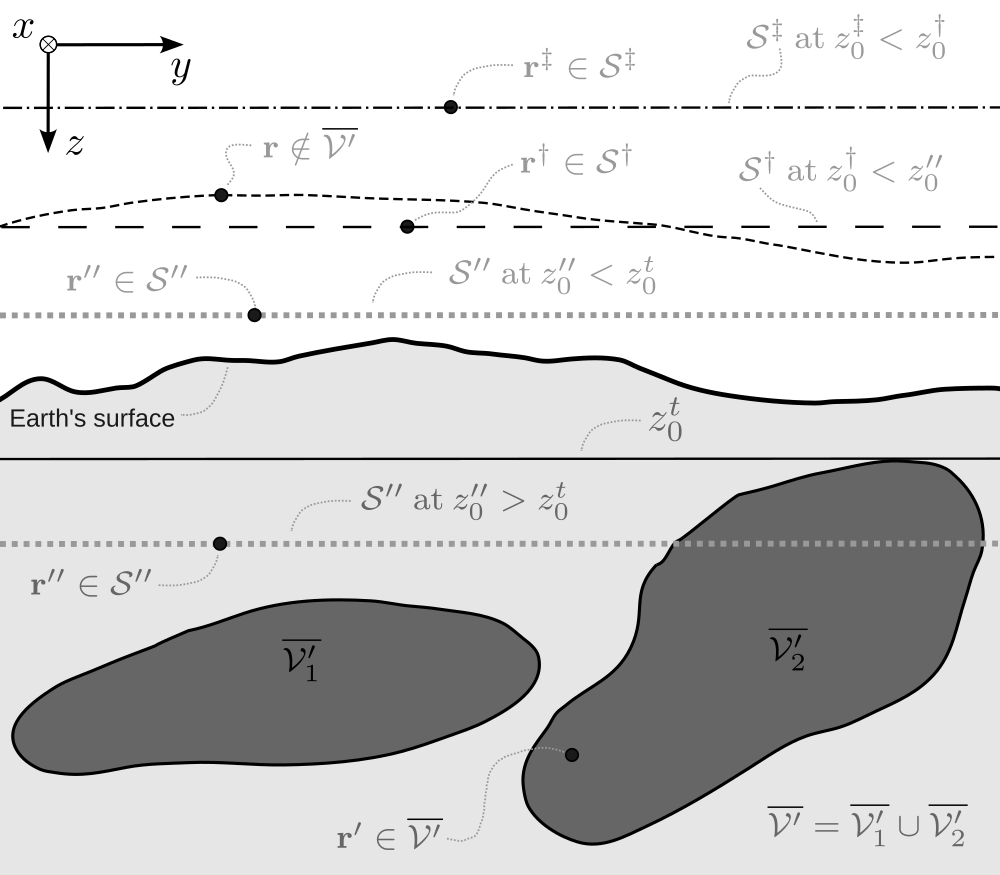
\includegraphics[width=0.8\textwidth]{figures/Figure1_1.png}
	\caption{%
		2D schematic representation of a vertical $yz$ plane crossing the sources (represented in dark gray),
		with $x$ axis pointing inward the page (represented by the ``$\otimes$" symbol).
		The sources are located in the subsurface (represented in light gray), over a 
		closed region $\overline{\mathcal{V}'}$ formed by $N_{\nu} = 2$ disjoint closed regions 
		$\overline{\mathcal{V}'_{\nu}}$, $\nu \in \{1, 2\}$, with top limited by the plane $z^{t}_{0}$. 
		The fine dashed lines represent two possible horizontal surfaces $\mathcal{S}''$, one located 
		at $z''_{0} < z^{t}_{0}$, above the sources, and another at $z''_{0} > z^{t}_{0}$, crossing the sources.
		The medium dashed line represents the surface containing the observation points 
		$\mathbf{r}$, all above $\mathcal{S}''$.
		The long dashed line represents a planar surface $\mathcal{S}^{\dagger}$ located 
		at $z^{\dagger}_{0} < z''_{0}$.
		Finally, the dashed-dot line represents a planar surface $\mathcal{S}^{\ddagger}$ located 
		at $z^{\ddagger}_{0} < z^{\dagger}_{0}$.
	}
	\label{fig:Figure1}
\end{figure}
\section{Continuous equivalent layers on a plane}
\label{eq:planar_eqlayer}

An equivalent layer is loosely defined as a physical property distribution that satisfactorily 
reproduces potential-field data and enables potential-field transformations. 
In the literature, equivalent layers are typically assumed to lie in source-free regions where 
Laplace’s equation holds. Consequently, it is presumed that the equivalent layer does not intersect 
the true sources. However, in practical applications, the positions of the true sources in the subsurface 
are often unknown, making this condition difficult to guarantee.
Empirical evidence suggests that equivalent-layer methods can still perform effectively 
when the layer intersects the sources \cite<e.g.,>[]{gonzalez_etal2022}.

In this section, we formally define \textit{continuous equivalent layers} 
on a horizontal surface $\mathcal{S}''$ that may either lie above or intersect the sources (Figure \ref{fig:Figure1}). 
Our goal is to leverage the properties of continuous layers to gain deeper insights into their discrete counterparts, 
which are explored in the companion paper 
``Planar equivalent layers for potential fields: 2. Geophysical implications and applications".

\begin{definition}[\textbf{Continuous equivalent layer}]
	Let us assume to have an observed potential field $d^{o}$ defined above 
	a horizontal surface $\mathcal{S}''$ with constant vertical coordinate $z''_{0}$. 
	Besides, consider (i) a horizontal surface $\mathcal{S}^{\dagger}$ that is located above 
	$\mathcal{S}''$, at a constant vertical coordinate $z^{\dagger}_{0}$, 
	and does not cross the sources and (ii) a harmonic kernel 
	$a$ that depends only on $\mathbf{r}$ and $\mathbf{r}'' \in \mathcal{S}''$, as well as 
	vanishes as the distance $\| \mathbf{r} - \mathbf{r}'' \|$ increases. 
	Then, for a chosen accuracy $\varepsilon > 0$, we may call $p_{\varepsilon}$ 
	a \underline{continuous equivalent layer} if its predicted potential field 
	\begin{equation}
		d_{\varepsilon}(\mathbf{r})
		= \int\limits_{-\infty}^{\infty}\int\limits_{-\infty}^{\infty}
		p_{\varepsilon}(\mathbf{r}'') \, a(\mathbf{r}, \mathbf{r}'') \:\: d\mathcal{S}''
		\: , \quad z < z''_{0} \: ,
		\label{eq:predicted-data-continuous-layer}
	\end{equation}
	satisfies 
	\begin{equation}
		\int\limits_{-\infty}^{\infty} \int\limits_{-\infty}^{\infty}
		\vert d^{o}(\mathbf{r}^{\dagger}) - 
		d_{\varepsilon}(\mathbf{r}^{\dagger}) \vert^{2}
		\:\: d\mathcal{S}^{\dagger} \le \varepsilon \: ,
		\quad z^{\dagger}_{0} < z^{t}_{0} \: , \quad z^{\dagger}_{0} < z''_{0} \: ,
		\label{eq:epsilon-bound-data}
	\end{equation}
	where $\mathbf{r} = (x, y, z)^{\top}$, 
	$\mathbf{r}^{\dagger} = (x^{\dagger}, y^{\dagger}, z^{\dagger}_{0})^{\top} \in \mathcal{S}^{\dagger}$ 
	and $\mathbf{r}'' = (x'', y'', z''_{0})^{\top} \in \mathcal{S}''$.
	\label{def:continuous-eqlayer}
\end{definition}

In Definition \ref{def:continuous-eqlayer}, $p_{\varepsilon}$ represents a 
continuous physical-property distribution that extends to infinity along the horizontal 
directions. 
Moreover, the kernel function $a$ is usually defined by $D_{a} \Psi$ 
as a generic partial derivative of $\Psi$ (equation \ref{eq:Psi}),
where $D_{a}$ is set in terms of the space-domain differential operator 
$D$ (equation \ref{eq:diff-operators-generic}).
It is important to stress here that the horizontal surface $\mathcal{S}''$ in 
Definition \ref{def:continuous-eqlayer} may cross the sources, according to 
Figure \ref{fig:Figure1}.

A particular continuous equivalent layer 
$p_{\varepsilon}$ leads to a transformed potential field given by:
\begin{equation}
	f_{\varepsilon}(\mathbf{r}^{\ddagger})
	= \int\limits_{-\infty}^{\infty}\int\limits_{-\infty}^{\infty}
	p_{\varepsilon}(\mathbf{r}'') \, t(\mathbf{r}^{\ddagger}, \mathbf{r}'') \:\: d\mathcal{S}'' \: , 
	\quad \mathbf{r}^{\ddagger} \in \mathcal{S}^{\ddagger} \: ,
	\quad \mathbf{r}'' \in \mathcal{S}'' \: ,
	\label{eq:transformed-field-continuous-layer}
\end{equation}
where $\mathbf{r}^{\ddagger}$ are points defined on a planar surface $\mathcal{S}^{\ddagger}$ located above 
$\mathcal{S}''$ (Figure \ref{fig:Figure1}); 
$f_{\varepsilon}$ is a transformed field that approximates $f$ (equations \ref{eq:transformed-field-space}); and
$t$ is the transformation kernel, which is usually defined by $D_{t} \Psi$ as a generic partial 
derivative of the potential function $\Psi$ (equation \ref{eq:Psi}), with $D_{t}$ given in terms of 
$D$ (equation \ref{eq:diff-operators-generic}).
In equation \ref{eq:transformed-field-continuous-layer}, we define $\mathbf{r}^{\ddagger}$ on 
a planar surface $\mathcal{S}^{\ddagger}$ located above $\mathcal{S}''$ (Figure \ref{fig:Figure1}), but this is not a 
restriction. They can coincide with the observation points or be arbitrarily defined above $\mathcal{S}''$.

\section{Existence of continuous equivalent layers on a plane}
\label{sec:planar_eqlayer_theorem}

\subsection{Modified Dirichlet's and Neumann's problems on a plane}

The classical solutions to Dirichlet’s and Neumann’s problems (Eq(s). \ref{eq:U-Dirichlet-Neumann} 
and \ref{eq:U-Dirichlet-Neumann-Fourier}) on a plane are specifically formulated for cases where 
the horizontal surface $\mathcal{S}''$ is positioned above the sources. In this section, we extend 
these classical solutions by removing this restriction and allowing $\mathcal{S}''$ to intersect 
the sources (Fig. \ref{fig:Figure1}).
 
We start by considering an auxiliary potential $U_{\varepsilon}$ that approximates $U$ (Eq. \ref{eq:potential-U-space})
at points $\mathbf{r} \notin \overline{\mathcal{V}'}$ above the sources, is square integrable on the surface 
$\mathcal{S}''$ and has a space domain representation given by 
\begin{equation}
	U_{\varepsilon}(\mathbf{r}) = 
	\int\limits_{-\infty}^{\infty} \int\limits_{-\infty}^{\infty}
	D(\ell, \hat{\mathbf{z}}) U_{\varepsilon}(\mathbf{r}'') \:\:
	D(1-\ell, \hat{\mathbf{z}}) \Psi(\mathbf{r}, \mathbf{r}'') 
	\:\: d\mathcal{S}'' \: , 
	\quad z < z^{t}_{0} \: , \quad z < z''_{0} \: ,
	\quad \ell \in \{ 0, 1 \} \: ,
	\label{eq:potential-U-epsilon-space}
\end{equation}
where $\mathbf{r} = (x, y, z)^{\top} \notin \overline{\mathcal{V}'}$; 
$\mathbf{r}'' = (x'', y'', z''_{0})^{\top} \in \mathcal{S}''$ (Fig. \ref{fig:Figure1}) and 
$D$ is the space-domain differential operator 
defined by Eq. \ref{eq:diff-operators-generic} in terms of the canonical base vector 
$\hat{\mathbf{z}}$ (Eq. \ref{eq:canonical-base-vector}).
We also consider that the Fourier-convolution theorem 
can be applied to the auxiliary potential $U_{\varepsilon}$
(Eq. \ref{eq:potential-U-epsilon-space}) on the horizontal surface $\mathcal{S}^{\dagger}$ above
the sources (Fig. \ref{fig:Figure1}), so that
\begin{equation}
	\mathcal{F} [ U_{\varepsilon}(\mathbf{r}^{\dagger}) ]
	= k \, \mathcal{F} [ U_{\varepsilon}(\mathbf{r}'') ] \:
	\mathcal{F} [ \Psi(\mathbf{r}^{\dagger}, \mathbf{r}'') ] \: ,
	\quad \mathbf{r}^{\dagger} \in \mathcal{S}^{\dagger} \: .
	\label{eq:potential-U-epsilon-Fourier-dagger}
\end{equation}
Using the definition of $\mathcal{F} [ \Psi(\mathbf{r}^{\dagger}, \mathbf{r}'') ]$ (Eq. \ref{eq:Psi-Fourier})
in Eq. \ref{eq:potential-U-epsilon-Fourier-dagger}, we conclude that $U_{\varepsilon}$ must satisfy
\begin{equation}
	\mathcal{F} [ U_{\varepsilon}(\mathbf{r}'') ] = 
	\mathcal{F} [ U_{\varepsilon}(\mathbf{r}^{\dagger}) ] \, e^{\, k \, (z''_{0} - z^{\dagger}_{0})} \: .
	\label{eq:potential-U-epsilon-Fourier-layer}
\end{equation}
Now we present two possible approaches to define an auxiliary potential $U_{\varepsilon}$ that satisfies the 
conditions above and lead to modified Dirichlet’s and Neumann’s problems that can be applied to 
the case in which $\mathcal{S}''$ cross the sources (Fig. \ref{fig:Figure1}). 

\subsubsection{Approach 1: Truncating wavenumber}

Let $U_{\varepsilon}$ be given by
\begin{equation}
	\mathcal{F} [ U_{\varepsilon}(\mathbf{r}^{\dagger}) ] = 
	\begin{cases}
		\mathcal{F} [ U(\mathbf{r}^{\dagger}) ] &
		, \quad 0 < k \le k_{\varepsilon} \\
		0 & , \quad k > k_{\varepsilon} 
	\end{cases} \: ,
	\label{eq:potential-U-epsilon-Fourier-dagger-1}
\end{equation}
where $k_{\varepsilon}$ is a fixed and possibly very large truncating wavenumber and 
$\mathcal{F} \left[ U(\mathbf{r}^{\dagger}) \right]$ is defined on the horizontal surface $\mathcal{S}^{\dagger}$ 
located above the sources (Fig. \ref{fig:Figure1}). 
As we can see, this definition of $U_{\varepsilon}$ 
(i) imposes that its Fourier transform coincides with 
that of $U$ (Eq. \ref{eq:potential-U-Fourier}) on the horizontal surface $\mathcal{S}^{\dagger}$ 
up to the truncating wavenumber $k_{\varepsilon}$; 
(ii) represents a smooth version of $U$ on $\mathcal{S}^{\dagger}$; and
(iii) leads to a square integrable function on $\mathcal{S}^{\dagger}$ because 
$U$ is square integrable on $\mathcal{S}^{\dagger}$ (Appendix \ref{app:upper-bounds}).
Then we obtain from Eq. \ref{eq:potential-U-epsilon-Fourier-layer} that 
\begin{equation}
	\mathcal{F} \left[ U_{\varepsilon}(\mathbf{r}'') \right] = 
	\begin{cases}
		\mathcal{F} \left[ U(\mathbf{r}^{\dagger}) \right] 
		e^{\, k \, (z''_{0} - z^{\dagger}_{0})} & , 
		\quad 0 < k \le k_{\varepsilon} \\
		0 & , \quad k > k_{\varepsilon} 
	\end{cases} \: ,
	\label{eq:potential-U-epsilon-Fourier-layer-1}
\end{equation}
which approximates the potential field obtained by 
computing the downward continuation of $U$ (Eq. \ref{eq:potential-U-space}) 
to points $\mathbf{r}'' \in \mathcal{S}''$ that may be located inside the sources (Fig. \ref{fig:Figure1}). 
It is well-known, however, that downward continuation can only be computed at 
source-free points, where the Laplace's equation applies. This means that the
continuation plane is limited by the top $z^{t}_{0}$ of the sources, otherwise the continued field 
presents an oscillatory character \citep[e.g.,][]{roy1967, fedi_florio2002} that may
prevent $\mathcal{F} \left[ U_{\varepsilon}(\mathbf{r}'') \right]$ to be square integrable.
The truncating wavenumber $k_{\varepsilon}$ used to define $U_{\varepsilon}$ according to Eq. 
\ref{eq:potential-U-epsilon-Fourier-layer-1} overcomes this problem, as suggested (but not shown) 
by \cite{bhattacharyya1967},
and guarantees that the Fourier-convolution theorem can be applied to Eq. \ref{eq:potential-U-epsilon-space} 
for obtaining Eq. \ref{eq:potential-U-epsilon-Fourier-dagger}.

At last, it can be easily verified that, if we let the truncating wavenumber $k_{\varepsilon}$ 
goes to infinity in Eq. \ref{eq:potential-U-epsilon-Fourier-layer-1} for the case in which 
$\mathcal{S}''$ is located above the sources, at $z''_{0} < z^{t}_{0}$ (Fig. \ref{fig:Figure1}), 
we get 
\begin{equation}
	\lim_{k_{\varepsilon}\to\infty} \mathcal{F} \left[ U_{\varepsilon}(\mathbf{r}'') \right] = 
	\mathcal{F} \left[ U(\mathbf{r}'') \right] \: , \quad z''_{0} < z^{t}_{0} \: ,
	\label{eq:lim-kepsilon-potential-U-epsilon-Fourier-layer}
\end{equation}
\begin{equation}
	\lim_{k_{\varepsilon}\to\infty} \mathcal{F} \left[ U_{\varepsilon}(\mathbf{r}^{\dagger}) \right] = 
	\mathcal{F} \left[ U(\mathbf{r}^{\dagger}) \right] \: , \quad z^{\dagger}_{0} < z''_{0} < z^{t}_{0} \: ,
	\label{eq:lim-kepsilon-potential-U-epsilon-Fourier-dagger}
\end{equation}
pointwise and, consequently, that
\begin{equation}
	\lim_{k_{\varepsilon}\to\infty} U_{\varepsilon}(\mathbf{r}) = 
	U(\mathbf{r}) \: , \quad z < z''_{0} < z^{t}_{0} \: ,
	\label{eq:lim-kepsilon-potential-U-epsilon-space}
\end{equation}
which is in perfect agreement with the classical solutions of the Dirichlet's and Neumann's
problems (Eq(s). \ref{eq:U-Dirichlet-Neumann} and \ref{eq:U-Dirichlet-Neumann-Fourier}).

\subsubsection{Approach 2: Tikhonov regularization}

We may also define $U_{\varepsilon}$ as the following smooth approximation of $U$ on the horizontal surface 
$\mathcal{S}^{\dagger}$ located above the sources (Fig. \ref{fig:Figure1}):
\begin{equation}
	\mathcal{F} [ U_{\varepsilon}(\mathbf{r}^{\dagger}) ] = 
	\tfrac{1}{1 + \mu_{\varepsilon} \, k^{2} \, e^{\, k \, (z''_{0} - z^{\dagger}_{0})}} \; 
	\mathcal{F} [ U(\mathbf{r}^{\dagger}) ] \: ,
	\label{eq:potential-U-epsilon-Fourier-dagger-2}
\end{equation}
where $\mu_{\varepsilon}$ is a fixed positive regularization parameter imposing smoothness on $U$ 
according to \cite{pasteka_etal2012}. 
Again, this proposed definition of $U_{\varepsilon}$ 
(i) represents a smooth version of $U$ on $\mathcal{S}^{\dagger}$ and
(ii) leads to a square integrable function on $\mathcal{S}^{\dagger}$.
Next, we obtain from Eq. \ref{eq:potential-U-epsilon-Fourier-layer} that 
\begin{equation}
	\mathcal{F} \left[ U_{\varepsilon}(\mathbf{r}'') \right] = 
	\tfrac{e^{\, k \, (z''_{0} - z^{\dagger}_{0})}}{1 + \mu_{\varepsilon} \, k^{2} \, e^{\, k \, (z''_{0} - z^{\dagger}_{0})}} \; 
	\mathcal{F} [ U(\mathbf{r}^{\dagger}) ] \: .
	\label{eq:potential-U-epsilon-Fourier-layer-2}
\end{equation}
The alternative definition of $U_{\varepsilon}$ given by Eq. \ref{eq:potential-U-epsilon-Fourier-dagger-2} 
also leads to an approximation of the potential field obtained by 
computing the downward continuation of $U$ (Eq. \ref{eq:potential-U-space}) 
to points $\mathbf{r}'' \in \mathcal{S}''$ that may be located inside the sources (Fig. \ref{fig:Figure1}). 
In this case, however, it is the regularization parameter $\mu_{\varepsilon}$ that forces  
$U_{\varepsilon}$ to be square integrable on $\mathcal{S}''$ and guarantees that the 
Fourier-convolution theorem can be applied to Eq. \ref{eq:potential-U-epsilon-space} 
for obtaining Eq. \ref{eq:potential-U-epsilon-Fourier-dagger}.

Finally, if we let the $\mu_{\varepsilon}$ 
goes to zero in Eq. \ref{eq:potential-U-epsilon-Fourier-layer-2} for the case in which 
$\mathcal{S}''$ is located above the sources, at $z''_{0} < z^{t}_{0}$ (Fig. \ref{fig:Figure1}), 
we obtain once more that 
\begin{equation}
	\lim_{\mu_{\varepsilon}\to 0} \mathcal{F} \left[ U_{\varepsilon}(\mathbf{r}'') \right] = 
	\mathcal{F} \left[ U(\mathbf{r}'') \right] \: , \quad z''_{0} < z^{t}_{0} \: ,
	\label{eq:lim-muepsilon-potential-U-epsilon-Fourier-layer}
\end{equation}
\begin{equation}
	\lim_{\mu_{\varepsilon}\to 0} \mathcal{F} \left[ U_{\varepsilon}(\mathbf{r}^{\dagger}) \right] = 
	\mathcal{F} \left[ U(\mathbf{r}^{\dagger}) \right] \: , \quad z^{\dagger}_{0} < z''_{0} < z^{t}_{0} \: ,
	\label{eq:lim-muepsilon-potential-U-epsilon-Fourier-dagger}
\end{equation}
pointwise and, consequently, that
\begin{equation}
	\lim_{\mu_{\varepsilon}\to 0} U_{\varepsilon}(\mathbf{r}) = 
	U(\mathbf{r}) \: , \quad z < z''_{0} < z^{t}_{0} \: ,
	\label{eq:lim-muepsilon-potential-U-epsilon-space}
\end{equation}
which is also in perfect agreement with the classical solutions of the Dirichlet's and Neumann's
problems (Eq(s). \ref{eq:U-Dirichlet-Neumann} and \ref{eq:U-Dirichlet-Neumann-Fourier}).

\subsubsection{On the physical interpretation of $U_{\varepsilon}$}

The auxiliary potential $U_{\varepsilon}$ on the surface $\mathcal{S}''$ is defined by Eq. 
\ref{eq:potential-U-epsilon-Fourier-layer-1}, in terms of a truncating wavenumber $k_{\varepsilon}$,
or Eq. \ref{eq:potential-U-epsilon-Fourier-layer-2}, in terms of a regularization parameter $\mu_{\varepsilon}$.
We emphasize that, when $\mathcal{S}''$ is located above the sources ($z''_{0} < z^{t}_{0}$, Fig. \ref{fig:Figure1}),
$U_{\varepsilon}$ is a smooth approximation of the potential $U$ (Eqs \ref{eq:potential-U-space} and \ref{eq:potential-U-Fourier}) 
due to the true sources.
However, when $\mathcal{S}''$ intersects the true sources ($z''_{0} > z^{t}_{0}$, Fig. \ref{fig:Figure1}), 
$U_{\varepsilon}$ (i) is a fictitious regularized harmonic continuation defined for the purpose of reproducing $U$ above the sources
and (ii) does not equal the actual non-harmonic Newtonian potential that a sensor would measure inside the sources.

\subsection{Formal existence demonstration of continuous layers}

In this subsection, we formally demonstrate the existence of planar equivalent layers 
$p_{\varepsilon}$ (Definition \ref{def:continuous-eqlayer}) 
through the formulation and proof of a theorem. This approach provides, for the first time, a rigorous mathematical 
framework for a concept traditionally based on empirical assumptions.
As the cornerstone of this study, the theorem moves beyond empirical assumptions to establish 
a mathematically sound basis for the well-known applications of the equivalent-layer technique, 
even for the case in which the layer crosses the sources.

\begin{theorem}[Planar equivalent-layer theorem]
	\label{theorem:planar-eqlayer-theorem}
	Let a horizontal surface $\mathcal{S}''$ and a kernel function $a$ 
	be set according to Definition \ref{def:continuous-eqlayer}, for a given observed potential field $d^{o}$. 
	Then, for every $\varepsilon > 0$, there exists a set of continuous equivalent layers $p_{\varepsilon}$ on $\mathcal{S}''$. 
	Furthermore, for the case in which $\mathcal{S}''$ is above the sources, the continuous equivalent layers 
	reproduce $d^{o}$ exactly.
\end{theorem}
\begin{proof}
	We start by defining $p_{\varepsilon}$ (Definition \ref{def:continuous-eqlayer}) 
	in the Fourier domain via
	\begin{equation}
		\mathcal{F} [ p_{\varepsilon}(\mathbf{r}'') ] =
		\tfrac{k \, \alpha_{d}}{\alpha_{a}} \,
		\mathcal{F} [ U_{\varepsilon}(\mathbf{r}'') ] \: ,
		\quad \mathbf{r}'' \in \mathcal{S}'' \: ,
		\label{eq:p-Fourier}
	\end{equation}
	where $\alpha_{a}$ is a differential operator 
	defined in the Fourier domain in terms of $\alpha$ (Eq. \ref{eq:diff-operators-generic}) and
	$U_{\varepsilon}$ is defined as in \ref{eq:potential-U-epsilon-Fourier-layer-1},
	for a given truncating wavenumber $k_{\varepsilon}$, or as in \ref{eq:potential-U-epsilon-Fourier-layer-2},
	for a given regularization parameter $\mu_{\varepsilon}$. 
	
	Note that there is an equivalent layer $p_{\varepsilon}$ for each particular $\alpha_{a}$.
	For any finite choice of $0 < k_{\varepsilon} < \infty$ or $0 < \mu_{\varepsilon} < \infty$
	(Eq(s). \ref{eq:potential-U-epsilon-Fourier-layer-1} and \ref{eq:potential-U-epsilon-Fourier-layer-2}), 
	both $\mathcal{F} [ p_{\varepsilon}(\mathbf{r}'') ]$ 
	and $p_{\varepsilon}(\mathbf{r}'')$ are square-integrable and, consequently, it is possible to
	apply the Fourier-convolution theorem to \ref{eq:predicted-data-continuous-layer} and obtain
	\begin{equation}
		\mathcal{F} [ d_{\varepsilon}(\mathbf{r}^{\dagger}) ] =
		\mathcal{F} [ p_{\varepsilon}(\mathbf{r}'') ] \, 
		\mathcal{F} [ a(\mathbf{r}^{\dagger}, \mathbf{r}'') ] \: ,
		\quad \mathbf{r}^{\dagger} \in \mathcal{S}^{\dagger} \: ,
		\quad \mathbf{r}'' \in \mathcal{S}'' \: ,
		\label{eq:predicted-data-continuous-layer-Fourier}
	\end{equation}
	where 
	\begin{equation}
		\mathcal{F} [ a(\mathbf{r}^{\dagger}, \mathbf{r}'') ] = \alpha_{a} \, \mathcal{F} [ \Psi(\mathbf{r}^{\dagger}, \mathbf{r}'') ] \: ,
		\quad \mathbf{r}^{\dagger} \in \mathcal{S}^{\dagger} \: ,
		\quad \mathbf{r}'' \in \mathcal{S}'' \: ,
		\label{eq:kernel-a-Fourier}
	\end{equation}
	with $a(\mathbf{r}, \mathbf{r}'') = D_{a} \Psi(\mathbf{r}, \mathbf{r}'')$;
	$\mathbf{r}^{\dagger} = (x^{\dagger}, y^{\dagger}, z^{\dagger}_{0})^{\top}$; 
	$\mathbf{r}'' = (x'', y'', z''_{0})^{\top}$ and $z^{\dagger}_{0} < z''_{0}$.
	By substituting equations \ref{eq:observed-data-Fourier}, \ref{eq:Psi-Fourier} and \ref{eq:kernel-a-Fourier} 
	into \ref{eq:predicted-data-continuous-layer-Fourier} and comparing the result with equations 
	\ref{eq:potential-U-epsilon-Fourier-layer-1} and \ref{eq:potential-U-epsilon-Fourier-layer-2}, 
	we find that $d_{\varepsilon}$ satisfies
	\begin{equation}
		\mathcal{F} [ d_{\varepsilon}(\mathbf{r}^{\dagger}) ] = 
		\alpha_{d} \,
		\mathcal{F} [ U_{\varepsilon}(\mathbf{r}^{\dagger}) ] \: ,
		\quad \mathbf{r}^{\dagger} \in \mathcal{S}^{\dagger} \: .
		\label{eq:predicted-data-continuous-layer-epsilon-Fourier}
	\end{equation}

	From Plancherel's theorem \citep[][p. 119]{bracewell1999} and use of polar coordinates 
	$k_{x} = k \, \cos\theta$, $k_{y} = k \, \sin\theta$ and $k = \sqrt{k_{x}^{2} + k_{y}^{2}}$,
	we get
	\begin{equation}
		\begin{split}
			\int\limits_{-\infty}^{\infty} \int\limits_{-\infty}^{\infty}
			\vert 
			d^{o}(\mathbf{r}^{\dagger}) - d_{\varepsilon}(\mathbf{r}^{\dagger})
			\vert^{2} 
			\: d\mathcal{S}^{\dagger} = 
			\int\limits_{-\infty}^{\infty} \int\limits_{-\infty}^{\infty}
			\vert \mathcal{F} [ d^{o}(\mathbf{r}^{\dagger}) ] - \mathcal{F} [
			d_{\varepsilon}(\mathbf{r}^{\dagger}) ] \vert^{2} 
			\: d k_{x} \, d k_{y} \\
			= \int\limits_{0}^{2\pi} \int\limits_{0}^{\infty}
			\vert \mathcal{F} [ d^{o}(\mathbf{r}^{\dagger}) ] - \mathcal{F} [
			d_{\varepsilon}(\mathbf{r}^{\dagger}) ] \vert^{2} \: k \: d k \, d \theta \: .
		\end{split}
		\label{eq:Plancherel}
	\end{equation}
	If we consider that the auxiliary potential $U_{\varepsilon}$ is defined by Eq. \ref{eq:potential-U-epsilon-Fourier-dagger-1},
	we obtain that 
	\begin{equation}
		\mathcal{F} [ d_{\varepsilon}(\mathbf{r}^{\dagger}) ] = 
		\begin{cases}
			\mathcal{F} [ d^{o}(\mathbf{r}^{\dagger}) ] &
			, \quad 0 < k \le k_{\varepsilon} \\
			0 & , \quad k > k_{\varepsilon} 
		\end{cases} \: .
		\label{eq:predicted-data-continuous-layer-epsilon-Fourier-1}
	\end{equation}
	If we now consider that $U_{\varepsilon}$ is given by Eq. \ref{eq:potential-U-epsilon-Fourier-dagger-2},
	we get
	\begin{equation}
		\mathcal{F} [ d_{\varepsilon}(\mathbf{r}^{\dagger}) ] = 
		\tfrac{1}{1 + \mu_{\varepsilon} \, k^{2} \, e^{\, k \, (z''_{0} - z^{\dagger}_{0})}} \; 
		\mathcal{F} [ d^{o}(\mathbf{r}^{\dagger}) ] \: .
		\label{eq:predicted-data-continuous-layer-epsilon-Fourier-2}
	\end{equation}
	It is important to note that using a finite but sufficiently large $0 < k_{\varepsilon} < \infty$ in Eq. 
	\ref{eq:predicted-data-continuous-layer-epsilon-Fourier-1} or a finite $0 < \mu_{\varepsilon} < \infty$ in 
	Eq. \ref{eq:predicted-data-continuous-layer-epsilon-Fourier-2} lead to  
	$\int_{0}^{2\pi} \int_{0}^{\infty} \vert \mathcal{F} [ d^{o}(\mathbf{r}^{\dagger}) ] - \mathcal{F} [d_{\varepsilon}(\mathbf{r}^{\dagger}) ] \vert^{2} \: k \, dkd\theta \le \varepsilon$ in Eq. \ref{eq:Plancherel}. 
	Because of that, we conclude that $p_{\varepsilon}$ (Eq. \ref{eq:p-Fourier})
	is a continuous equivalent layer according to Definition \ref{def:continuous-eqlayer}. 
	Besides, if the layer plane is above the sources (i.e., if $z''_{0} < z^{t}_{0}$), then both 
	$\mathcal{F} [ p_{\varepsilon}(\mathbf{r}'') ]$ and $p_{\varepsilon}(\mathbf{r}'')$ are square-integrable
	even for the choice $k_{\varepsilon} = \infty$ or $\mu_{\varepsilon} = 0$. Then, in that case, 
	$\int_{0}^{2\pi} \int_{0}^{\infty} 
	\vert \mathcal{F} [ d^{o}(\mathbf{r}^{\dagger}) ] - \mathcal{F} [d_{\varepsilon}(\mathbf{r}^{\dagger}) ] \vert^{2} \: k \, dkd\theta 
	= 0$ and $p_{\varepsilon}$ yields a predicted field $d_{\varepsilon}$ that exactly reproduces the observed field $d^{o}$ 
	on $\mathcal{S}^{\dagger}$.
\end{proof}

\begin{remark}
	\label{rm:remark0}
	In Eq. \ref{eq:p-Fourier}, $\alpha_{d}$ and $\alpha_{a}$ are algebraic polynomials of 
	$\mathbf{k} = ( \mathtt{i} \, k_{x} \, , \, \mathtt{i} \, k_{y} \, , \, k)^{\top}$ (Eq. \ref{eq:diff-operators-generic})
	representing linear combinations of spatial directional derivatives.
	When $\alpha_{a} = 0$ at specific wavenumbers $k_{x}$ and $k_{y}$, division by $\alpha_{a}$ introduces division-by-zero 
	issues. These potential problems are controlled because $\alpha_{a}$ acts on the auxiliary potential 
	$U_{\varepsilon}$ given by Eq. \ref{eq:potential-U-epsilon-Fourier-layer-1}, for a given truncating wavenumber $k_{\varepsilon}$, 
	or Eq. \ref{eq:potential-U-epsilon-Fourier-layer-2}, for a given regularization parameter $\mu_{\varepsilon}$. 
	These truncation/regularization approaches guarantee that the quotient $\tfrac{\alpha_{d}}{\alpha_{a}} \mathcal{F}[U_\epsilon]$ remains 
	well-defined, square-integrable, and numerically stable.
\end{remark}
	
\begin{remark}
	\label{rm:remark1}
	The planar equivalent-layer theorem guarantees the existence of a planar and continuous equivalent layer, even if
	it crosses the sources, i.e., if $z''_{0} > z^{t}_{0}$ (Fig. \ref{fig:Figure1}).
	But it does not provide any guidance on the particular choice of the 
	truncating wavenumber $k_{\varepsilon}$ (Eq. \ref{eq:potential-U-epsilon-Fourier-dagger-1}) or the 
	regularization parameter $\mu_{\varepsilon}$ (Eq. \ref{eq:potential-U-epsilon-Fourier-dagger-2}) 
	for the construction of $p_{\varepsilon}$, with a given accuracy level 
	$\varepsilon$ (Definition \ref{def:continuous-eqlayer}).
\end{remark}

\begin{remark}
	\label{rm:remark2}
	The truncating wavenumber $k_{\varepsilon}$ and the regularization parameter $\mu_{\varepsilon}$ 
	play a central role in the planar equivalent-layer theorem (Theorem \ref{theorem:planar-eqlayer-theorem}). 
	Both parameters impose smoothness on the planar equivalent layer. 
	In practical situations, the interpreter usually estimate a ``sufficiently smooth'' discrete equivalent layer 
	that ``satisfactorily'' fit the observed data within a given error level. 
	It seems that this discretization and the imposed degree of smoothness are important factors rendering 
	the equivalent-layer technique even when the layer plane crosses the sources.
	From a theoretical point of view, it might be interesting to study the influence of
	discretizing continuous equivalent layers and its relation to $k_{\varepsilon}$ and $\mu_{\varepsilon}$. 
	We implicitly assume that the estimated discrete layer obtained in a practical situation 
	approximates the corresponding continuous layer $p_{\varepsilon}$ (Definition \ref{def:continuous-eqlayer}) as the discretization becomes increasingly finer. 
	This assumption is confirmed by the numerical tests we present in the companion paper 
	``Planar equivalent layers for potential fields: 2. Geophysical implications and applications" .
\end{remark}

\begin{remark}
	\label{rm:remark3}
	Any continuous equivalent layer $p_{\varepsilon}$ (Definition \ref{def:continuous-eqlayer}) leads to a predicted 
	potential field that satisfies
	the error bound $\varepsilon$ (Eq. \ref{eq:epsilon-bound-data}) not only on the surface $\mathcal{S}^{\dagger}$, but also 
	on any $\mathcal{S}^{\ddagger}$ with $z^{\ddagger}_{0} < z^{\dagger}_{0}$ (Fig. \ref{fig:Figure1}). 
	Namely, it follows from Eq. \ref{eq:potential-U-Fourier} that
	\begin{equation}
		\int\limits_{-\infty}^{\infty} \int\limits_{-\infty}^{\infty}
		\vert d^{o}(\mathbf{r}^{\ddagger}) - d_{\varepsilon}(\mathbf{r}^{\ddagger})
		\vert^{2} \: d\mathcal{S}^{\ddagger} \le
		\int\limits_{-\infty}^{\infty} \int\limits_{-\infty}^{\infty}
		\vert d^{o}(\mathbf{r}^{\dagger}) - d_{\varepsilon}(\mathbf{r}^{\dagger})
		\vert^{2} \: d\mathcal{S}^{\dagger} \: ,
		\quad z^{\ddagger}_{0} < z^{\dagger}_{0} \: .
		\label{eq:error-bound-upper-planes}
	\end{equation}
	Thus, if $p_{\varepsilon}$ produces a $d_{\varepsilon}$ satisfying 
	$\int_{-\infty}^{\infty} \int_{-\infty}^{\infty} \vert d^{o}(\mathbf{r}^{\dagger}) - d_{\varepsilon}(\mathbf{r}^{\dagger}) 
	\vert^{2} \: d\mathcal{S}^{\dagger} \le \varepsilon$, then it automatically holds that 
	$\int_{-\infty}^{\infty} \int_{-\infty}^{\infty} \vert d^{o}(\mathbf{r}^{\ddagger}) - d_{\varepsilon}(\mathbf{r}^{\ddagger}) 
	\vert^{2} \: d\mathcal{S}^{\ddagger} \le \varepsilon$.
\end{remark}


\section{Unified approach for potential-field transformations}

Given a particular equivalent layer $p_{\varepsilon}$ (Definition \ref{def:continuous-eqlayer}) 
defined as a square-integrable function by equation \ref{eq:p-Fourier}, in terms of specific $\alpha_{d}$ and $\alpha_{a}$, 
it is theoretically possible to compute any potential field transformation (equations \ref{eq:transformed-field-space} and 
\ref{eq:transformed-field-Fourier}).
It means that, contrarily to the common sense, we do not need to use a planar layer of dipoles to compute the RTP anomaly from 
the approximated total-field anomaly, for example. In fact, even a layer of monopoles can be used to perform this potential-field transformation. 
This can be verified by first noting that applying the Fourier-convolution theorem to \ref{eq:transformed-field-continuous-layer} 
on a planar surface $\mathcal{S}^{\ddagger}$ (Figure \ref{fig:Figure1}) gives
\begin{equation}
	\mathcal{F} [ f_{\varepsilon}(\mathbf{r}^{\ddagger}) ] =
	\mathcal{F} \left[ p_{\varepsilon}(\mathbf{r}'') \right]
	\mathcal{F} [ t(\mathbf{r}^{\ddagger}, \mathbf{r}'') ] \: , 
	\quad \mathbf{r}^{\ddagger} \in \mathcal{S}^{\ddagger} \: ,
	\quad \mathbf{r}'' \in \mathcal{S}'' \: ,
	\label{eq:transformed-field-continuous-layer-Fourier}
\end{equation}
where
\begin{equation}
	\mathcal{F} [ t(\mathbf{r}^{\ddagger}, \mathbf{r}'') ] = \alpha_{t} \, \mathcal{F} [ \Psi(\mathbf{r}^{\ddagger}, \mathbf{r}'') ]
	\label{eq:kernel-t-Fourier}
\end{equation}
is defined in terms of a differential operator $\alpha_{t}$ acting on $\Psi$ (equation \ref{eq:Psi}) in the Fourier domain.
Then we set 
\begin{equation}
	\alpha_{t} = \left( \tfrac{\alpha_{a}}{\alpha_{d}} \right) \alpha_{f} \: ,
	\label{eq:alpha-t-generic}
\end{equation}
where $\alpha_{f}$ is the differential operator associated with the desired potential field $f$ (equation \ref{eq:transformed-field-Fourier}).
In this case, we get from equations \ref{eq:Psi-Fourier}, \ref{eq:p-Fourier}  and \ref{eq:kernel-t-Fourier} 
that the transformed potential field $f_{\varepsilon}$ (equation \ref{eq:transformed-field-continuous-layer-Fourier}) 
is given by:
\begin{equation}
	\mathcal{F} [ f_{\varepsilon}(\mathbf{r}^{\ddagger}) ] =
	\alpha_{f} \, k \, \mathcal{F} [ U_{\varepsilon}(\mathbf{r}'') ] \: 
	\mathcal{F} [ \Psi(\mathbf{r}^{\ddagger}, \mathbf{r}'') ] \: , 
	\quad \mathbf{r}^{\ddagger} \in \mathcal{S}^{\ddagger} \: ,
	\quad \mathbf{r}'' \in \mathcal{S}'' \: .
	\label{eq:transformed-field-continuous-layer-Fourier2}
\end{equation}
Finally, we use \ref{eq:Psi-Fourier}, \ref{eq:transformed-field-Fourier} and \ref{eq:potential-U-epsilon-Fourier-layer} to show that
\begin{equation}
	\mathcal{F} [ f_{\varepsilon}(\mathbf{r}^{\ddagger}) ] = 
	\begin{cases}
		\mathcal{F} [ f(\mathbf{r}^{\ddagger}) ] &
		, \quad 0 < k \le k_{\varepsilon} \\
		0 & , \quad k > k_{\varepsilon} 
	\end{cases} \: ,
	\label{eq:transformed-field-continuous-layer-1-Fourier}
\end{equation}
if the auxiliary potential $U_{\varepsilon}$ is defined by equation \ref{eq:potential-U-epsilon-Fourier-dagger-1},
or
\begin{equation}
	\mathcal{F} [ f_{\varepsilon}(\mathbf{r}^{\ddagger}) ] = 
	\tfrac{1}{1 + \mu_{\varepsilon} \, k^{2} \, e^{\, k \, (z''_{0} - z^{\ddagger}_{0})}} \; 
	\mathcal{F} [ f(\mathbf{r}^{\ddagger}) ] \: ,
	\label{eq:transformed-field-continuous-layer-2-Fourier}
\end{equation}
if the auxiliary potential $U_{\varepsilon}$ is defined by equation \ref{eq:potential-U-epsilon-Fourier-dagger-2}.
In both cases, we can see that the transformed field $f_{\varepsilon}$ yielded by the equivalent layer 
is a smooth approximation of that produced by the true sources on the planar surface $\mathcal{S}^{\ddagger}$
(Figure \ref{fig:Figure1}). Note that, to obtain a correct potential-field transformation leading to an $f_{\varepsilon}$ 
that approximates $f$, we need to correctly set the operator $\alpha_{t}$ (equation \ref{eq:alpha-t-generic}), 
regardless of the equivalent layer type defined by $\alpha_{a}$.


In the context of the equivalent-layer technique, a potential-field transformation is generally defined
in the space domain, by following two steps. The first consists in obtaining a particular layer $p_{\varepsilon}$ 
(Definition \ref{def:continuous-eqlayer}), which is subsequently used to compute a transformed field $f_{\varepsilon}$ via 
\ref{eq:transformed-field-continuous-layer}.
It can be verified, however, that this two-step approach is equivalent to the single-step approach based on the 
Fourier transform of the observed potential field (equation \ref{eq:field-transformation-Fourier}). 
We find by using \ref{eq:observed-data-Fourier} and \ref{eq:transformed-field-continuous-layer-Fourier2} that
\begin{equation}
	\mathcal{F} [ f_{\varepsilon}(\mathbf{r}^{\ddagger}) ] =
	\left( \tfrac{\alpha_{f}}{\alpha_{d}} \right) \, \mathcal{F} [ d_{\varepsilon}(\mathbf{r}^{\ddagger}) ]
	 \: .
	\label{eq:transformed-field-continuous-layer-single-step}
\end{equation}
Then, if we consider that the predicted field $d_{\varepsilon}$ (equation \ref{eq:predicted-data-continuous-layer-epsilon-Fourier})
is defined in terms of the auxiliary potential $U_{\varepsilon}$ given by equation \ref{eq:potential-U-epsilon-Fourier-dagger-1},
we get
\begin{equation}
	\mathcal{F} [ f_{\varepsilon}(\mathbf{r}^{\ddagger}) ] =
	\left( \tfrac{\alpha_{f}}{\alpha_{d}} \right) \, 
	\begin{cases}
		\mathcal{F} \left[ d^{o}(\mathbf{r}^{\dagger}) \right] 
		e^{\, k \, (z^{\ddagger}_{0} - z^{\dagger}_{0})} & , \quad 0 < k \le k_{\varepsilon} \\
		0 & , \quad k > k_{\varepsilon} 
	\end{cases} \: .
	\label{eq:transformed-field-continuous-layer-1-single-step}
\end{equation}
Alternatively, if we consider that the predicted field $d_{\varepsilon}$ (equation \ref{eq:predicted-data-continuous-layer-epsilon-Fourier})
is defined in terms of the auxiliary potential $U_{\varepsilon}$ given by equation \ref{eq:potential-U-epsilon-Fourier-dagger-2},
we get
\begin{equation}
	\mathcal{F} [ f_{\varepsilon}(\mathbf{r}^{\ddagger}) ] =
	\left( \tfrac{\alpha_{f}}{\alpha_{d}} \right) \, 
	\tfrac{1}{1 + \mu_{\varepsilon} \, k^{2} \, e^{\, k \, (z''_{0} - z^{\dagger}_{0})}} \;
	\mathcal{F} \left[ d^{o}(\mathbf{r}^{\dagger}) \right] \: .
	\label{eq:transformed-field-continuous-layer-2-single-step}
\end{equation}
Note that, for the particular case in which $z^{\ddagger}_{0}$ coincides with $z^{\dagger}_{0}$ and 
the truncating wavenumber $k_{\varepsilon}$ goes to infinity, equation 
\ref{eq:transformed-field-continuous-layer-1-single-step} reduces to \ref{eq:field-transformation-Fourier}.
Similarly, if $z^{\ddagger}_{0}$ coincides with $z^{\dagger}_{0}$ and $\mu_{\varepsilon}$ goes to zero,
equation \ref{eq:transformed-field-continuous-layer-2-single-step} also reduces to \ref{eq:field-transformation-Fourier}.
For the first time, we provide a mathematical proof establishing the link between
potential-field transformations performed using the equivalent-layer technique in 
the space domain and those computed via Fourier transformation of the observed data.
This connection sheds light on why potential-field transformations based on the
equivalent layers can exhibit the same numerical instabilities commonly associated
with Fourier-based transformations of potential-field data. This
relationship is widely acknowledged and is typically justified, without any proof, by  
the notion that physical phenomena are independent of the domain 
-- whether spatial or Fourier -- used for their computation.
\section{Equivalent layer classes}
\label{sec:eqlayer_classes}

According to the Planar Equivalent-Layer Theorem (Theorem \ref{theorem:planar-eqlayer-theorem}), 
it is possible to define different planar equivalent layers $p_{\varepsilon}$, 
$\mathbf{r}'' \in \mathcal{S}''$ (Fig.\ref{fig:Figure1}), 
satisfying the conditions imposed by Definition \ref{def:continuous-eqlayer}.
Specifically, different equivalent layers $p_{\varepsilon}$ can be defined
on the same horizontal surface $\mathcal{S}''$, for the same potential field $d^{o}$, 
by using different combinations of $\alpha_{d}$ and $\alpha_{a}$ in Eq. \ref{eq:p-Fourier}. 
The horizontal surface $\mathcal{S}''$ may be located above the sources 
or intersect them (Fig.\ref{fig:Figure1}).
Here we show different classes of equivalent layers, discuss their applicability and define how they 
can be used to perform potential-field transformations.

\subsection{Dirichlet's equivalent layers}

\begin{definition}
	An equivalent layer $p_{\varepsilon}$ (Definition \ref{def:continuous-eqlayer}) is called Dirichlet's equivalent 
	layer if it has the following form in the Fourier domain:
	\begin{equation}
		\mathcal{F} [ p_{\varepsilon}(\mathbf{r}'') ] =
		\alpha_{d} \, \mathcal{F} [ U_{\varepsilon}(\mathbf{r}'') ]  \: .
		\label{eq:p-Fourier-Dirichlet}
	\end{equation}
	\label{def:eql-Dirichlet}
\end{definition}
Note that Dirichlet's layers (Definition \ref{def:eql-Dirichlet}) are obtained from 
Eq. \ref{eq:p-Fourier} by setting $\alpha_{a} \equiv \alpha(1, \hat{\mathbf{z}}) = k$ 
(Eq. \ref{eq:diff-operators-generic}).
In this case, we can easily verify from equations \ref{eq:observed-data-Fourier},
\ref{eq:potential-U-epsilon-Fourier-layer-1} and \ref{eq:potential-U-epsilon-Fourier-layer-2} that they 
approximate the downward continuation of the observed potential field $d^{o}$ to the layer plane $\mathcal{S}''$.
It is important noting that such layers depend on $\alpha_{d}$, which 
carries information about the observed potential field (Eq. \ref{eq:observed-data-Fourier}).
In this case, the corresponding predicted field (Eq. \ref{eq:predicted-data-continuous-layer}) assumes the form
\begin{equation}
	d_{\varepsilon}(\mathbf{r})
	= \int\limits_{-\infty}^{\infty}\int\limits_{-\infty}^{\infty}
	p_{\varepsilon}(\mathbf{r}'') \: \tfrac{\partial}{\partial z} \Psi(\mathbf{r}, \mathbf{r}'') \:\: d\mathcal{S}''
	\: , \quad z < z''_{0} \: .
	\label{eq:predicted-data-Dirichlet-layer}
\end{equation}
From the physical point of view, this $d_{\varepsilon}$ is analogous
to the vertical component of the gravitational attraction due to a layer of monopoles
or the magnetic scalar potential due to a layer of vertically-magnetized dipoles.
Moreover, Eq. \ref{eq:predicted-data-Dirichlet-layer} approximates the well-known \textit{upward continuation integral} 
\citep[e.g.,][]{skeels1947, peters1949, henderson-zietz1949, dean1958, roy1962, bhattacharyya1967, henderson1970},
which is traditionally derived from the solution of the Dirichlet’s problem on the
layer plane (Eq. \ref{eq:U-Dirichlet-Neumann} with $\ell = 0$). 

Dirichlet's equivalent layers are the basis of the pioneer method proposed by \cite{dampney1969} for processing gravity data.
Such layers lead to potential-field transformations (Eq(s). 
\ref{eq:transformed-field-continuous-layer} and \ref{eq:transformed-field-continuous-layer-Fourier}) defined by 
$\alpha_{t} = \nicefrac{k \, \alpha_{f}}{\alpha_{d}}$ (Eq. \ref{eq:alpha-t-generic}).
Dirichlet's equivalent layers are commonly used to perform upward/downward continuation of the observed potential 
field, which is obtained by setting $\alpha_{f} = \alpha_{d}$, resulting in $\alpha_{t} = k$. 
Other potential-field transformations can also be accomplished from such equivalent layers, but they must be 
defined in terms of $\alpha_{f} \ne \alpha_{d}$.
In this case, however, defining the resulting transformed field $f_{\varepsilon}$ explicitly in the space domain 
(Eq. \ref{eq:transformed-field-continuous-layer}) 
from its counterpart in the Fourier domain (Eq. \ref{eq:transformed-field-continuous-layer-Fourier}) may be very difficult.


\subsection{Equivalent layers having minimum phase changes}

\begin{definition}
	An equivalent layer $p_{\varepsilon}$ (Definition \ref{def:continuous-eqlayer}) is said to have minimum 
	phase changes (with respect to the spatial distribution of the true sources) if its phase spectrum is given by
	\begin{equation}
		\Theta [ p_{\varepsilon}(\mathbf{r}'') ] = \Theta [ U_{\varepsilon}(\mathbf{r}^{\dagger}) ] \: ,
		\label{eq:p-phase-spectrum-U}
	\end{equation}
	where $\Theta [ U_{\varepsilon}(\mathbf{r}^{\dagger}) ]$ denotes the phase spectrum of $U_{\varepsilon}$ 
	(Appendix \ref{app:potential-U-min-phase}, equations \ref{eq:potential-U-epsilon-1-phase-spectrum} and \ref{eq:potential-U-epsilon-2-phase-spectrum}).
	\label{def:eql-min-phase}
\end{definition}
\begin{proposition}
	\label{prop:minimum-phase-change-layers}
	An equivalent layer $p_{\varepsilon}$ having minimum phase changes (Definition \ref{def:eql-min-phase})
	depends only on the spatial distribution of the true sources and not on the particular observed 
	potential field $d^{o}$.
\end{proposition}
\begin{proof}
	It follows from equations \ref{eq:p-phase-spectrum-U} and definition of phase spectrum (Appendix \ref{app:potential-U-min-phase}) that 
	$\mathcal{F} [ p_{\varepsilon}(\mathbf{r}'') ]$ must be the product of a real function and
	$\mathcal{F} [ U_{\varepsilon}(\mathbf{r}^{\dagger}) ]$.
	From equations \ref{eq:potential-U-epsilon-Fourier-layer} and \ref{eq:p-Fourier}, we can verify that 
	$\mathcal{F} [ p_{\varepsilon}(\mathbf{r}'') ]$ is in fact the product of 
	$\mathcal{F} [ U_{\varepsilon}(\mathbf{r}^{\dagger}) ]$ 
	and a term $\left( \nicefrac{\alpha_{d}}{\alpha_{a}} \right) k \, e^{\, k \, (z''_{0} - z^{\dagger}_{0})}$. 
	Since $\nicefrac{\alpha_{d}}{\alpha_{a}}$ is the only term that can be a complex function, we conclude that 
	the imposed condition can only be satisfied for the case in which $\alpha_{a} = \alpha_{r} \, \alpha_{d}$, 
	where $\alpha_{r}$ is a generic real function satisfying $\alpha_{r} \ne 0$ for $0 < k \le k_{\varepsilon}$.
	It can then be verified that, in this case, \ref{eq:p-Fourier} assumes the form
	\begin{equation}
		\mathcal{F} [ p_{\varepsilon}(\mathbf{r}'') ] =
		\tfrac{k}{\alpha_{r}} \, \mathcal{F} [ U_{\varepsilon}(\mathbf{r}^{\dagger}) ] 
		e^{\, k \, (z''_{0} - z^{\dagger}_{0})} \: ,
		\label{eq:p-Fourier-min-phase}
	\end{equation}
	which is the product of a real function and $\mathcal{F} [ U_{\varepsilon}(\mathbf{r}^{\dagger}) ]$.
	Since $\alpha_{r}$ does not depend on $\alpha_{d}$, $\mathcal{F} [ p_{\varepsilon}(\mathbf{r}'') ]$ does not 
	depend on $\alpha_{d}$ as well. This implies that the phase spectrum of $p_{\varepsilon}$ approximates that 
	of the potential $U$ (Appendix \ref{app:potential-U-min-phase}), thereby corresponding to an approximation 
	of the phase spectrum associated with the spatial distribution of the (shallow parts of the) true sources.
\end{proof}

Equivalent layers having minimum phase changes (Definition \ref{def:eql-min-phase}) may present intricate 
spatial domain representations, dictated by the particular form of the real function $\alpha_{r}$
(Eq. \ref{eq:p-Fourier-min-phase}).
Such layers give raise to potential-field transformations (Eq. \ref{eq:transformed-field-continuous-layer-Fourier})
defined by $\alpha_{t} = \alpha_{r} \, \alpha_{f}$ (Eq. \ref{eq:alpha-t-generic}), which may also
have non-trivial representations in the space domain.

\subsection{Neumann's equivalent layers}

\begin{definition}
	An equivalent layer $p_{\varepsilon}$ (Definition \ref{def:continuous-eqlayer}) is called Neumann's equivalent 
	layer if it has the following form in the Fourier domain:
	\begin{equation}
		\mathcal{F} [ p_{\varepsilon}(\mathbf{r}'') ] =
		k \, \mathcal{F} [ U_{\varepsilon}(\mathbf{r}'') ] \: .
		\label{eq:p-Fourier-Neumann}
	\end{equation}
	\label{def:eql-Neumann}
\end{definition}
\begin{proposition}
	All Neumann's equivalent layers have minimum phase changes.
	\label{prop:eql-Neumann}
\end{proposition}
\begin{proof}
	Equation \ref{eq:p-Fourier-Neumann} is directly obtained from \ref{eq:p-Fourier}, by using 
	$\alpha_{a} = \alpha_{d}$. It can be easily verified that, in this case, 
	$\mathcal{F} [ p_{\varepsilon}(\mathbf{r}'') ]$ is a particular case of Eq. \ref{eq:p-Fourier-min-phase},
	with $\alpha_{r} = 1$. Consequently, Neumann's equivalent layers have minimum phase changes
	according to Definition \ref{def:eql-min-phase}.
\end{proof}

The predicted potential field $d_{\varepsilon}$ (Eq. \ref{eq:predicted-data-continuous-layer}) 
due to Neumann's equivalent layers (Definition \ref{def:eql-Neumann}) assumes the form
\begin{equation}
	d_{\varepsilon}(\mathbf{r})
	= \int\limits_{-\infty}^{\infty}\int\limits_{-\infty}^{\infty}
	p_{\varepsilon}(\mathbf{r}'') \: D_{d} \Psi(\mathbf{r}, \mathbf{r}'') \:\: d\mathcal{S}''
	\: , \quad z < z''_{0} \: ,
	\label{eq:predicted-data-Neumann-layer}
\end{equation}
where $D_{d}$ is the same space-domain differential operator associated with
the observed potential field $d^{o}$ (Eq. \ref{eq:observed-data-space}).
As a consequence, Neumann's equivalent layers (Definition \ref{def:eql-Neumann}) preserve the physical
relationship between the observed potential field and the true sources.
It means that, if the observed potential field $d^{o}$ is the $x$-component of the 
gravitational attraction due to the true sources, the predicted potential field $d_{\varepsilon}$  
represents the $x$-component of the gravitational attraction due to the planar equivalent layer, for example.
The same is valid for any other potential field.

Any particular Neumann's layer $p_{\varepsilon}$ yields transformed potential 
fields (Eq. \ref{eq:transformed-field-continuous-layer-Fourier}) 
defined by $\alpha_{t} = \alpha_{f}$ (Eq. \ref{eq:alpha-t-generic}) in the Fourier domain. 
Hence, the corresponding transformed field $f_{\varepsilon}$ in the space domain 
(Eq. \ref{eq:transformed-field-continuous-layer}) assumes the simple form
\begin{equation}
	f_{\varepsilon}(\mathbf{r})
	= \int\limits_{-\infty}^{\infty}\int\limits_{-\infty}^{\infty}
	p_{\varepsilon}(\mathbf{r}'') \: D_{f} \Psi(\mathbf{r}, \mathbf{r}'') \:\: d\mathcal{S}''
	\: , \quad z < z''_{0} \: ,
	\label{eq:transformed-field-continuous-layer-Neumann}
\end{equation}
where $D_{f}$ is the space-domain representation of the differential operator $\alpha_{f}$ 
associated with the desired transformed field $f$ (Eq. \ref{eq:transformed-field-space}).

It follows immediately from Eq. \ref{eq:p-Fourier-Neumann} that Neumann's equivalent layers approximate 
the vertical derivative $\tfrac{\partial}{\partial z} U$ (Eq. \ref{eq:potential-U-1st-deriv-space}) 
on the layer plane $\mathcal{S}''$.
For the cases in which the observed potential field $d^{o}$ represents gravity data, 
$p_{\varepsilon}$ approximates the gravity disturbance (or vertical component of the gravitational
attraction) due to the true sources on the layer plane $\mathcal{S}''$.
If $d^{o}$ represents magnetic data produced by sources with constant total magnetization direction, 
then $p_{\varepsilon}$ approximates the pseudogravity 
anomaly \citep[][p. 345]{blakely1996} due to the true sources on $\mathcal{S}''$.
In this case, $p_{\varepsilon}$ is strictly positive because it is defined in terms of a strictly positive 
function $\sigma$ (Eq. \ref{eq:potential-U-space}) representing the 
total-magnetization intensity at all points 
$\mathbf{r}' = (x', y', z')^{\top} \in \overline{\mathcal{V}'}$ 
within the sources.
This result is in perfect agreement with that deduced by \cite{reis_etal2020} for
the particular case in which the observed potential field $d^{o}$ is
the approximated total-field anomaly (Table \ref{tbl:Table1}).

It is widely known that integrating the potential field $\tfrac{\partial}{\partial z} U$ 
(Eq. \ref{eq:potential-U-1st-deriv-space}) on a horizontal plane above the causative sources
gives their total mass (or total dipole moment), according to the
Gauss' theorem \citep[e.g.,][]{hammer1945, lafehr1965, bhattacharyya1967}. 
Furthermore, \cite{medeiros-silva1995a} show that the horizontal first-order moments, second-order moment $xy$, 
difference between the second-order moments $xx$ and $yy$, as well as the horizontal coordinates of the sources center of mass
(or center of dipole moment) of the true sources can also be estimated from the $\tfrac{\partial}{\partial z} U$
that they produce on a horizontal plane above them.
Thus, all these parameters of the true sources can be directly estimated from 
Neumann's equivalent layers $p_{\varepsilon}$ (Definition \ref{def:eql-Neumann}) because
they approximate the field $\tfrac{\partial}{\partial z} U$ (Eq. \ref{eq:potential-U-1st-deriv-space}) 
on $\mathcal{S}''$.
\section{Conclusions}
\label{sec:conclusions}

We furnish the theoretical background for potential-field transformations
that have been empirically made in space domain by using equivalent layers since 
this technique was introduced in applied geophysics during the 1960s.
Our goal here is to replace the widely accepted equivalent-layer principle, which 
refers to the empirical generalizations
by which most of the studies found in the geophysical literature justify the existence of
equivalent layers allowing the computation of potential-field transformations.
Specifically, we have presented the planar equivalent-layer theorem to state
the existence of planar and continuous equivalent layers that 
reproduce the potential-field data exactly when they reside strictly in the source-free 
region above the sources, or within a predefined error level when they intersect the true sources.
We have proven this mathematical statement by modifying the solutions of the 
Dirichlet's and Neumann's problems on planar surfaces that may cross the sources.
We also establish how a particular equivalent layer can be used to perform a particular 
potential-field transformation.
Furthermore, we define the theoretical link between potential-field transformations made 
via the equivalent-layer technique and those directly computed from the Fourier transform of the observed 
potential-field data. 
In essence, we have filled the theoretical gaps in most of the existing equivalent-layer 
methods and have also shown that a planar equivalent layer is not a purely mathematical abstraction,
but carries physical meaning and is directly related to boundary value problems of potential 
theory.
We contribute to the general understanding on why the technique has long been 
successfully applied to perform potential-field transformations. 
Our work opens the door for future theoretical investigations about potential-field 
transformations via the equivalent-layer technique, as well as for the relationship between 
planar equivalent layers and the true sources.

%%% End of body of article

%%%%%%%%%%%%%%%%%%%%%%%%%%%%%%%%%%%%%%%%%%%%%%%
%% Optional Appendices go here
%
% The \appendix command resets counters and redefines section heads
%
% After typing \appendix
%
%\section{Here Is Appendix Title}
% will show
% A: Here Is Appendix Title

\appendix
%\section{Here is a sample appendix}
\section{Some useful upper bounds}
\label{app:upper-bounds}

Here we define upper bounds for the absolute values
of $\mathcal{F} [ U(\mathbf{r}^{\dagger}) ]$ and $\mathcal{F} [ d^{o}(\mathbf{r}^{\dagger}) ]$ 
(equations \ref{eq:potential-U-Fourier} and \ref{eq:observed-data-Fourier}), 
i.e., for the amplitude spectra of $U$ and $d^{o}$ 
(equations \ref{eq:potential-U-space} and \ref{eq:observed-data-space}). 
To do this, we have adapted the approach presented by
\citeA{bhattacharyya1967} to define an upper bound for the amplitude spectrum of 
$\tfrac{\partial}{\partial z} U$. 
We first stress that 
$e^{- k \, (z' - z^{\dagger}_{0})} \le e^{- k \, (z^{t}_{0} - z^{\dagger}_{0})}$ because
$z^{t}_{0} \le z'$, where $z^{t}_{0}$ defines the top of the sources and $z'$ the vertical
coordinate of a point inside the sources. Using this identity in  
$\mathcal{F} [ U(\mathbf{r}^{\dagger}) ]$ (equation \ref{eq:potential-U-Fourier}), we obtain
\begin{equation}
	\vert \mathcal{F} [ U(\mathbf{r}^{\dagger}) ] \vert \le 2 \pi \kappa 
	\frac{e^{- k \, \Delta z}}{k}
	\int\limits_{z^{t}_{0}}^{\infty}
	\mathcal{F} [ \sigma(\mathbf{r}') ] \:
	\: dz' \: , \quad \Delta z = z^{t}_{0} - z^{\dagger}_{0} > 0 \: .
	\label{eq:potential-U-spectrum-bound1}
\end{equation}
This equation is valid because we assume that $\sigma$ (equation \ref{eq:potential-U-space}) 
is an integrable scalar function that is zero at all points $\mathbf{r}' \notin \overline{\mathcal{V}}$, 
where $\overline{\mathcal{V}}$ has a finite extension. 
Manipulating $\mathcal{F} [ \sigma(\mathbf{r}') ]$ (equation \ref{eq:sigma-Fourier}), 
we obtain
\begin{equation}
	\vert \mathcal{F} [ \sigma(\mathbf{r}') ] \vert \le
	\int\limits_{-\infty}^{\infty}\int\limits_{-\infty}^{\infty}
	\vert \sigma(\mathbf{r}') \vert 
	\: dx'dy'
	\label{eq:sigma-spectrum-bound}
\end{equation}
and, consequently, that
\begin{equation}
	2 \pi \kappa \, 
	\int\limits_{z^{t}_{0}}^{\infty}
	\vert \mathcal{F} [ \sigma(\mathbf{r}') ] \vert
	\: dz' \le \Omega \: ,
	\label{eq:Omega-bound}
\end{equation}
where
\begin{equation}
	\Omega = 2 \pi \kappa \, \iiint\limits_{\mathcal{V}}
	\vert \sigma(\mathbf{r}') \vert 
	\: d\mathcal{V}'
	\label{eq:Omega}
\end{equation}
is a constant depending only on the position and shape of the sources. 
Then, by combining equations 
\ref{eq:potential-U-spectrum-bound1}--\ref{eq:Omega},
we conclude that the amplitude spectrum of 
$U$ (equation \ref{eq:potential-U-space}) on a horizontal plane 
$z^{\dagger}_{0} < z^{t}_{0}$ located above the sources satisfies 
\begin{equation}
	\vert \mathcal{F} [ U(\mathbf{r}^{\dagger}) ] \vert \le
	\frac{e^{- k \, \Delta z}}{k} \, \Omega \: ,
	\: \quad \Delta z = z^{t}_{0} - z^{\dagger}_{0} > 0 \: .
	\label{eq:potential-U-spectrum-bound}
\end{equation}
From the upper bound of $\vert \mathcal{F} [ U(\mathbf{r}^{\dagger}) ] \vert$
(equation \ref{eq:potential-U-spectrum-bound}) and $\mathcal{F} [ d^{o}(\mathbf{r}^{\dagger}) ]$
(equation \ref{eq:observed-data-Fourier}), we also deduce
\begin{equation}
	\vert \mathcal{F} [ d^{o}(\mathbf{r}^{\dagger}) ] \vert \le
	\vert \alpha_{d} \vert \, \Omega \, 
	\frac{e^{- k \, \Delta z}}{k} \: ,
	\: \quad \Delta z = z^{t}_{0} - z^{\dagger}_{0} > 0 \: .
	\label{eq:observed-data-spectrum-bound}
\end{equation}
Note that, for the case in which $\alpha_{d} = k$ (equation \ref{eq:observed-data-Fourier}), 
we obtain the same result presented by \citeA{bhattacharyya1967} as the upper bound for the 
amplitude spectrum of $\tfrac{\partial}{\partial z} U$, whereas
$\alpha_{d} = 1$ leads to the upper bound defined by equation \ref{eq:potential-U-spectrum-bound}.
Equations \ref{eq:potential-U-spectrum-bound} and \ref{eq:observed-data-spectrum-bound} 
show that the amplitude spectra 
$\vert \mathcal{F} [ U(\mathbf{r}^{\dagger}) ] \vert$ and 
$\vert \mathcal{F} [ d^{o}(\mathbf{r}^{\dagger}) ] \vert$ on a plane $z^{\dagger}_{0} < z^{t}_{0}$ 
above the sources 
(i) are finite at all wavenumbers $k = \sqrt{k_{x}^{2} + k_{y}^{2}}$ and (ii) tend
to zero as $k$ goes to infinite.
These results confirm the well-known fact that 
$\mathcal{F} [ U(\mathbf{r}^{\dagger}) ]$ and $\mathcal{F} [ d^{o}(\mathbf{r}^{\dagger}) ]$ 
(equations \ref{eq:potential-U-Fourier} and \ref{eq:observed-data-Fourier}) are square integrable.
\section{Phase spectrum of the potentials $U$ and $U_{\varepsilon}$}
\label{app:potential-U-min-phase}

Let the phase spectrum \citep[e.g.,][p. 261]{blakely1996} of  
$\mathcal{F} [ U(\mathbf{r}^{\dagger}) ]$ (Eq. \ref{eq:potential-U-Fourier}) 
on a horizontal plane $z^{\dagger}_{0}$ above the sources be defined as follows:
\begin{equation}
	\Theta [ U(\mathbf{r}^{\dagger}) ] = \tan^{-1} \left( 
	\frac{\text{Im} \, \mathcal{F} [ U(\mathbf{r}^{\dagger}) ]}{\text{Re} \, \mathcal{F} [ U(\mathbf{r}^{\dagger}) ]} 
	\right) \: ,
	\label{eq:potential-U-phase-spectrum}
\end{equation}
where ``$\text{Re}$'' and ``$\text{Im}$'' denote the real and imaginary parts, respectively.

According to Eq. \ref{eq:potential-U-phase-spectrum}, the phase spectrum of $U$ (Eq. \ref{eq:potential-U-Fourier}) 
represents a weighted sum of the Fourier transforms $\mathcal{F} [ \sigma(\mathbf{r}') ]$
(Eq. \ref{eq:sigma-Fourier}) over all depth slices crossing the sources,
where the weights are real functions that exponentially decay with depth $z'$.
It means that $\Theta [ U(\mathbf{r}^{\dagger}) ]$ attributes more weight to the shallow than to the deeper parts of the sources. 
Because of that, the phase spectrum of $U$ approximates that of $\sigma$ and, consequently, 
$U$ has approximately the same horizontal spatial distribution of the (shallow parts of) true sources.
The same reasoning can be applied to the phase spectra of any vertical integral or vertical derivative of the potential $U$.

It can be easily verified that, for the case in which $U_{\varepsilon}$ is given by Eq. 
\ref{eq:potential-U-epsilon-Fourier-dagger-1} in the Fourier domain, we have that
\begin{equation}
	\Theta [ U_{\varepsilon}(\mathbf{r}'') ] = \begin{cases}
		\Theta [ U(\mathbf{r}^{\dagger}) ] & , \quad 0 < k \le k_{\varepsilon} \\
		0 & , \quad k > k_{\varepsilon}
	\end{cases} \: .
	\label{eq:potential-U-epsilon-1-phase-spectrum}
\end{equation}
It can also be easily verified that, for the case in which $U_{\varepsilon}$ is given by Eq. 
\ref{eq:potential-U-epsilon-Fourier-dagger-2} in the Fourier domain, we have that
\begin{equation}
	\Theta [ U_{\varepsilon}(\mathbf{r}'') ] = \Theta [ U(\mathbf{r}^{\dagger}) ] \: .
	\label{eq:potential-U-epsilon-2-phase-spectrum}
\end{equation}

%%%%%%%%%%%%%%%%%%%%%%%%%%%%%%%%%%%%%%%%%%%%%%%
% Optional Glossary, Notation or Acronym section goes here:
%
% Glossary is only allowed in Reviews of Geophysics
%  \begin{glossary}
%  \term{Term}
%   Term Definition here
%  \term{Term}
%   Term Definition here
%  \term{Term}
%   Term Definition here
%  \end{glossary}


%%%%%%%%%%%%%%%%%%%%%%%%%%%%%%%%%%%%%%%%%%%%%%%
% Acronyms
%% NOTE that acronyms in the final published version will be spelled out when used in figure captions.
%   \begin{acronyms}
%   \acro{Acronym}
%   Definition here
%   \acro{EMOS}
%   Ensemble model output statistics
%   \acro{ECMWF}
%   Centre for Medium-Range Weather Forecasts
%   \end{acronyms}


%%%%%%%%%%%%%%%%%%%%%%%%%%%%%%%%%%%%%%%%%%%%%%%
% Notation
%   \begin{notation}
%   \notation{$a+b$} Notation Definition here
%   \notation{$e=mc^2$}
%   Equation in German-born physicist Albert Einstein's theory of special
%  relativity that showed that the increased relativistic mass ($m$) of a
%  body comes from the energy of motion of the body—that is, its kinetic
%  energy ($E$)—divided by the speed of light squared ($c^2$).
%   \end{notation}




%%%%%%%%%%%%%%%%%%%%%%%%%%%%%%%%%%%%%%%%%%%%%%%
%
% DATA SECTION and ACKNOWLEDGMENTS
%
%%%%%%%%%%%%%%%%%%%%%%%%%%%%%%%%%%%%%%%%%%%%%%%

\section*{Open Research Section}
This section MUST contain a statement that describes where the data supporting the conclusions can be obtained. Data cannot be listed as ''Available from authors'' or stored solely in supporting information. Citations to archived data should be included in your reference list. Wiley will publish it as a separate section on the paper’s page. Examples and complete information are here:
https://www.agu.org/Publish with AGU/Publish/Author Resources/Data for Authors

%\section*{As Applicable – Inclusion in Global Research Statement}
%The Authorship: Inclusion in Global Research policy aims to promote greater equity and transparency in research collaborations. AGU Publications encourage research collaborations between regions, countries, and communities and expect authors to include their local collaborators as co-authors when they meet the AGU Publications authorship criteria (described here: https://www.agu.org/publications/authors/policies\#authorship). Those who do not meet the criteria should be included in the Acknowledgement section. We encourage researchers to consider recommendations from The TRUST CODE - A Global Code of Conduct for Equitable Research Partnerships (https://www.globalcodeofconduct.org/) when conducting and reporting their research, as applicable, and encourage authors to include a disclosure statement pertaining to the ethical and scientific considerations of their research collaborations in an “Inclusion in Global Research Statement’ as a standalone section in the manuscript following the Conclusions section. This can include disclosure of permits, authorizations, permissions and/or any formal agreements with local communities or other authorities, additional acknowledgements of local help received, and/or description of end-users of the research. You can learn more about the policy in this editorial. Example statements can be found in the following published papers: 
%Holt et al. (https://agupubs.onlinelibrary.wiley.com/doi/full/10.1029/2022JG007188), 
%Sánchez-Gutiérrez et al. (https://agupubs.onlinelibrary.wiley.com/doi/abs/10.1029/2023JG007554), 
%Tully et al. (https://agupubs.onlinelibrary.wiley.com/doi/epdf/10.1029/2022JG007128) 
%Please note that these statements are titled as “Global Research Collaboration Statements” from a previous pilot requirement in JGR Biogeosciences. The pilot has ended and statements should now be titled “Inclusion in Global Research Statement”.

\section*{Conflict of Interest disclosure}
The authors declare there are no conflicts of interest for this manuscript.


\acknowledgments
Enter acknowledgments here. This section is to acknowledge funding, thank colleagues, enter any secondary affiliations, and so on.




%%%%%%%%%%%%%%%%%%%%%%%%%%%%%%%%%%%%%%%%%%%%%%%
% REFERENCES and BIBLIOGRAPHY
%
% \bibliography{<name of your .bib file>} don't specify the file extension
% don't specify bibliographystyle
%
%%%%%%%%%%%%%%%%%%%%%%%%%%%%%%%%%%%%%%%%%%%%%%%

\bibliography{references}



%Reference citation instructions and examples:
%
% Please use ONLY \cite and \citeA for reference citations.
% \cite for parenthetical references
% ...as shown in recent studies (Simpson et al., 2019)
% \citeA for in-text citations
% ...Simpson et al. (2019) have shown...
%
%
%...as shown by \citeA{jskilby}.
%...as shown by \citeA{lewin76}, \citeA{carson86}, \citeA{bartoldy02}, and \citeA{rinaldi03}.
%...has been shown \cite{jskilbye}.
%...has been shown \cite{lewin76,carson86,bartoldy02,rinaldi03}.
%... \cite <i.e.>[]{lewin76,carson86,bartoldy02,rinaldi03}.
%...has been shown by \cite <e.g.,>[and others]{lewin76}.
%
% apacite uses < > for prenotes and [ ] for postnotes
% DO NOT use other cite commands (e.g., \citet, \citep, \citeyear, \nocite, \citealp, etc.).
%


\end{document}


